\section{Inoculation tests on European grapevine
  varieties}\label{app:inoculations}

\textbf{Plants}. Grapevine saplings were annually supplied from a nursery in
mainland Spain (Viveros Villanueva Vides, SL), consisting of one-year-old
rootstocks grafted in winter with dormant grapevine cultivars, and grown in
20-L plastic pots with a standard potting mix. Fifty-seven rootstock-scion
cultivar combinations were used in the inoculation assay (\cref{tableS1}).
Potted plants were randomly distributed in 12-plant rows along an insect-proof
tunnel exposed to air temperature and daily dip-irrigated to field capacity,
fortnightly sprinkled with a slow-release fertiliser and treated with
insecticides and fungicides when needed until the end of the experiment. Two
weeks before the onset of the inoculation assay, leaf samples of all plants
were collected and tested for the presence of Xf through qPCR as described
elsewhere \cite{Moralejo2019}.\\

\noindent\textbf{Isolates and inoculation}. We used for the inoculation
experiment two isolates of Xf. subsp. \textit{fastidiosa} (ST1) recovered from
grapevines: XLY 2055/17 (GenBank WGS: QTJS01) and XYL2177/18 (JAAGVM01)
\cite{Gomila2019,Moralejo2020}. In the third-year assay, we included an isolate
of Xf subsp. \textit{multiplex} ST81 XYL1981/18 (JAAGV1) to test whether
other strains in Majorca could cause PD as well. Isolates were grown on BYCE
medium at 28ºC for 7-10 days, following EPPO protocols \cite{EPPO2018}.  Cells
were collected by scraping the colonies and suspending them in 1.5 ml Eppendorf
tubes each with 1 ml o1f phosphate-buffered saline (PBS) solution until
obtaining a turbid ($10^8-10^9$ cell/ml) suspension. Plants were mechanically
inoculated by pin-prick inoculation \cite{Almeida2003} with slight
modifications. A 10-$\mu l$ drop of the bacterial suspension was pipetted on
the leaf axil and punctured five times with an entomological needle.
Eight-nine replicates per scion-rootstock combination were inoculated with the
bacterial suspension and four-three plants per cultivar with a drop of PBS as a
control at the end of May. Inoculation was repeated two weeks thereafter by
piercing the next leaf axil above that previously inoculated
\cite{Moralejo2019}.\\

\noindent\textbf{Disease score.} Disease severity was rated by counting the
number of symptomatic leaves eight weeks post-inoculation (WPI) and then
biweekly until the 16th week. A disease index was calculated according to Su et
al. \cite{Su2013}. To determine the basipetal and systemic movement of
Xf$_{\textrm{PD}}$, we counted the number of symptomatic leaves below the point
of inoculation from the same stems or any stem below at 12 WPI. Symptomatic and
asymptomatic plants were tested by qPCR for Xf infection at 12 WPI taking the
petiole of the second and fifth leaf above the point of inoculation. On the
14th week, five leaves per plant of all inoculated plants were used for
Xf$_{\textrm{PD}}$ isolation, as described below. Those plants for which the
qPCR was negative and Xf$_{\textrm{PD}}$ could not be isolated were treated as
not infected.\\

\noindent\textbf{Data analysis}. All statistical analyses on disease scores
were carried out using R. 3.5.2 version software
\cite{R-Development-Core-Team2017}. We used the functions glm and glmer in the
R package lme4 \cite{Bates2015}  for fitting Generalised Linear Models and
Generalised Linear Mixed Models (GLMMs) in the analysis of disease incidence
and severity in the inoculation assays. In all tests, we modelled the response
variable (i) disease incidence with the binomial error (logit‐link function)
and (ii) disease severity with the Poisson error (log‐link function). A
within-subject (repeated measures) factorial design was performed to evaluate
differences in disease severity over time among different cultivar-rootstock
combinations. Cultivars-rootstock and time were treated as fixed factors and
plant subjects as a random effect. Rootstock and time were analysed as fixed
factors and plant subjects as a random effect. Controls were excluded from the
analysis, as lesions did not develop on them. For each cultivar, we calculated
the area under the disease progress curve (AUDPC) from weeks-post-inoculation
and disease index using the package Agricolae. To test whether genotypes within
the ST1-grapevine population vary in virulence, we included a second strain
(XYL2177/18) in the 2019 inoculation experiment.\\

\noindent\textbf{Varietal response to Xf}. In our three-year inoculation tests,
we included a representative number of local and international varieties
(\cref{tableS1}). In total, among 886 inoculated-grapevine plants comprising 36
varieties in 57 unique combinations (scion-rootstock), 86.1\% ($n = 764$) of
them developed typical PD symptoms at 16 WPI. In contrast, none of the
grapevine plants inoculated with the strain XYL 1981/17, ST81 subsp.
\textit{multiplex} presented symptoms. The results of the pathogenicity tests
on European grape varieties are shown in \cref{tableS1}.

\begin{longtblr}[
    caption = {\textbf{Summary of the inoculation tests on grapevine varieties
                ranked from most to less susceptible in the disease index.}
            Thirty-six local,
            regional and international varieties were screened in combination
            with eight
            rootstocks. The number of symptomatic leaves was counted 16 weeks
            after
            inoculation and infections were confirmed by qPCR. DI: disease
            index; AUDCP:
            area under the disease progress curve.},
    label = {tableS1},
    ]{
    width = \linewidth,
    colspec = {Q[246]Q[138]Q[140]Q[62]Q[27]Q[104]Q[140]Q[69]},
    column{2} = {c},
    column{3} = {c},
    column{4} = {c},
    column{5} = {c},
    column{6} = {c},
    cell{1}{7} = {c},
    cell{1}{8} = {c},
    cell{2}{7} = {c},
    cell{2}{8} = {c},
    cell{3}{7} = {c},
    cell{3}{8} = {c},
    cell{4}{7} = {c},
    cell{4}{8} = {c},
    cell{5}{7} = {c},
    cell{5}{8} = {c},
    cell{6}{7} = {c},
    cell{6}{8} = {c},
    cell{7}{7} = {c},
    cell{7}{8} = {c},
    cell{8}{7} = {c},
    cell{8}{8} = {c},
    cell{9}{7} = {c},
    cell{10}{7} = {c},
    cell{10}{8} = {c},
    cell{11}{7} = {c},
    cell{11}{8} = {c},
    cell{12}{7} = {c},
    cell{12}{8} = {c},
    cell{13}{7} = {c},
    cell{13}{8} = {c},
    cell{14}{7} = {c},
    cell{14}{8} = {c},
    cell{15}{7} = {c},
    cell{15}{8} = {c},
    cell{16}{7} = {c},
    cell{16}{8} = {c},
    cell{17}{7} = {c},
    cell{17}{8} = {c},
    cell{18}{7} = {c},
    cell{18}{8} = {c},
    cell{19}{7} = {c},
    cell{19}{8} = {c},
    cell{20}{7} = {c},
    cell{20}{8} = {c},
    cell{21}{7} = {c},
    cell{21}{8} = {c},
    cell{22}{7} = {c},
    cell{22}{8} = {c},
    cell{23}{7} = {c},
    cell{23}{8} = {c},
    cell{24}{7} = {c},
    cell{24}{8} = {c},
    cell{25}{7} = {c},
    cell{25}{8} = {c},
    cell{26}{7} = {c},
    cell{26}{8} = {c},
    cell{27}{7} = {c},
    cell{27}{8} = {c},
    cell{28}{7} = {c},
    cell{28}{8} = {c},
    cell{29}{7} = {c},
    cell{29}{8} = {c},
    cell{30}{7} = {c},
    cell{30}{8} = {c},
    cell{31}{8} = {c},
    cell{32}{7} = {c},
    cell{32}{8} = {c},
    cell{33}{7} = {c},
    cell{33}{8} = {c},
    cell{34}{7} = {c},
    cell{34}{8} = {c},
    cell{35}{7} = {c},
    cell{35}{8} = {c},
    cell{36}{7} = {c},
    cell{36}{8} = {c},
    cell{37}{8} = {c},
    cell{38}{7} = {c},
    cell{38}{8} = {c},
    cell{39}{7} = {c},
    cell{39}{8} = {c},
    cell{40}{7} = {c},
    cell{40}{8} = {c},
    cell{41}{7} = {c},
    cell{41}{8} = {c},
    cell{42}{7} = {c},
    cell{42}{8} = {c},
    cell{43}{7} = {c},
    cell{43}{8} = {c},
    cell{44}{7} = {c},
    cell{44}{8} = {c},
    cell{45}{7} = {c},
    cell{45}{8} = {c},
    cell{46}{7} = {c},
    cell{46}{8} = {c},
    cell{47}{7} = {c},
    cell{47}{8} = {c},
    cell{48}{7} = {c},
    cell{48}{8} = {c},
    cell{49}{7} = {c},
    cell{49}{8} = {c},
    cell{50}{7} = {c},
    cell{50}{8} = {c},
    cell{51}{7} = {c},
    cell{51}{8} = {c},
    cell{52}{7} = {c},
    cell{52}{8} = {c},
    cell{53}{7} = {c},
    cell{53}{8} = {c},
    cell{54}{7} = {c},
    cell{54}{8} = {c},
    cell{55}{8} = {c},
    cell{56}{7} = {c},
    cell{56}{8} = {c},
    cell{57}{8} = {c},
    cell{58}{7} = {c},
    cell{58}{8} = {c},
    cell{59}{7} = {c},
    cell{59}{8} = {c},
    cell{60}{7} = {c},
    cell{60}{8} = {c},
    cell{61}{7} = {c},
    cell{61}{8} = {c},
    cell{62}{7} = {c},
    cell{62}{8} = {c},
    cell{63}{7} = {c},
    cell{63}{8} = {c},
    cell{64}{8} = {c},
    cell{65}{7} = {c},
    cell{65}{8} = {c},
    cell{66}{7} = {c},
    cell{66}{8} = {c},
    cell{67}{7} = {c},
    cell{67}{8} = {c},
    cell{68}{7} = {c},
    cell{68}{8} = {c},
    cell{69}{7} = {c},
    cell{69}{8} = {c},
    cell{70}{7} = {c},
    cell{70}{8} = {c},
    cell{71}{7} = {c},
    cell{71}{8} = {c},
    cell{72}{7} = {c},
    cell{72}{8} = {c},
    cell{73}{7} = {c},
    cell{73}{8} = {c},
    cell{74}{8} = {c},
    hline{75} = {-}{},
    } \hline
    \textbf{Scion}     & \textbf{Rootstock} & \textbf{Nº leaves} & \textbf{DI}
    &
    & \textbf{AUDCP} & \textbf{\% Positive} & \textbf{Year} \\ \hline
    Gorgollassa      & R110		  & 24.5 ± 8.8	       & 5.00	     &
    & 31.29	 & 100			& 2018		\\
    Sauvignon Blanc    & R110		  & 16.5 ± 3.3	       & 5.00	     &
    & 28.37	 & 100			& 2018		\\
    Tempranillo      & SO4		  & 15.7 ± 4.0	       & 5.00	     &
    & 37.22	 & 100			& 2019		\\
    Garnacha tintorera & R110		  & 19.0 ± 7.4	       & 5.00	     &
    & 32.17	 & 94.44		& 2019		\\
    Tempranillo      & 41B		  & 13.8 ± 2.7	       & 4.89	     &
    & 13.43	 & 0.00 		& 2020		\\
    Syrah	     & R140		  & 13.6 ±3.0	       & 4.86	     &
    & 29.46	 & 98.21		& 2019		\\
    Tempranillo Blanco & R110		  & 16.0 ± 4.9	       & 4.83	     &
    & 41.61	 & 94.44		& 2019		\\
    Chardonnay	     & R110		  & 16.6 ± 5.6	       & 4.83	     &
    & 26.39	 & 94.44		& 2019		\\
    Bobal	     & R110		  & 15.2 ± 6.8	       & 4.78	     &
    & 25.44	 & 94.44		& 2019		\\
    Prensal	     & 161/49		  & 15.7 ± 5.0	       & 4.75	     &
    & 21.37	 & 100			& 2018		\\
    Viura	     & SO4		  & 16.7 ± 4.7	       & 4.75	     &
    & 26.25	 & 100			& 2018		\\
    Garnacha tintorera & P1103		  & 15.8 ± 6.8	       & 4.72	     &
    & 35.94	 & 94.44		& 2019		\\
    Graciano	     & R140		  & 14.3 ± 5.6	       & 4.61	     &
    & 22.44	 & 88.89		& 2019		\\
    Airen	     & R110		  & 15.2 ± 5.9	       & 4.61	     &
    & 23.06	 & 94.44		& 2019		\\
    Mandó	     & R110		  & 11 ± 3.6	       & 4.56	     &
    & 21.22	 & 100			& 2018		\\
    Tempranillo      & R110 RJ43	  & 11.9 ± 3.0	       & 4.56	     &
    & 31.17	 & 100			& 2019		\\
    Tempranillo      & R110 RJ78	  & 11.7 ± 3.8	       & 4.50	     &
    & 34.33	 & 94.44		& 2019		\\
    Tempranillo      & 41B		  & 12.4 ± 4.7	       & 4.44	     &
    & 26.06	 & 61.11		& 2019		\\
    Garnacha	     & R110		  & 11.1 ± 3.4	       & 4.44	     &
    & 25.00	 & 83.33		& 2019		\\
    Viura	     & P1103		  & 20.3 ± 8.4	       & 4.37	     &
    & 25.875	 & 87.5 		& 2018		\\
    Malvasia	     & R110		  & 13.8 ± 6.5	       & 4.33	     &
    & 26.71	 & 71.73		& 2019		\\
    Tempranillo      & R110 RJ43	  & 12.2 ± 5.9	       & 4.33	     &
    & 24.23	 & 88.89		& 2020		\\
    Pedro Ximenez      & R140		  & 10.0 ± 4.33        & 4.33	     &
    & 16.87	 & 0.00 		& 2020		\\
    Hondarrabi Beltza  & 196-17 	  & 11.2 ± 4.6	       & 4.22	     &
    & 19.90	 & 87.5 		& 2019		\\
    Tempranillo      & P1103		  & 12.7 ± 6.3	       & 4.17	     &
    & 30.62	 & 62.5 		& 2018		\\
    Albariño	     & R110		  & 9.5 ± 4.3	       & 4.06	     &
    & 24.50	 & 66.67		& 2019		\\
    Garnacha tintorera & P1103		  & 13.1 ± 8.0	       & 4.0	     &
    & 16.85	 & 88.89		& 2020		\\
    Tempranillo      & R110		  & 11.7 ± 7.0	       & 3.94	     &
    & 26.72	 & 77.78		& 2019		\\
    Merlot	     & R110		  & 16.4  ± 13.1       & 3.75	     &
    & 24.87	 & 75			& 2018		\\
    Manto Negro      & R110		  & 11.9 ± 3.1	       & 3.75	     &
    & 16.37	 &			& 2018		\\
    Macabeo (Viura)    & R110		  & 13.0 ±9.6	       & 3.72	     &
    & 19.54	 & 70.83		& 2019		\\
    Pinot Noir	     & R110		  & 10.3 ± 7.1	       & 3.67	     &
    & 13.42	 & 44.44		& 2020		\\
    Tempranillo Blanco & R110		  & 11.2 ± 8.4	       & 3.56	     &
    & 17.31	 & 55.56		& 2020		\\
    Syrah	     & R110		  & 9.0 ± 5.6	       & 3.50	     &
    & 12.37	 & 100			& 2018		\\
    Verdejo	     & R110		  & 9.5 ± 6.6	       & 3.50	     &
    & 13.89	 & 72.22		& 2019		\\
    Airen	     & R110		  & 8.7 ± 5.3	       & 3.44	     &
    & 15.98	 &			& 2020		\\
    Monastrell	     & R110		  & 12.3 ± 8.8	       & 3.39	     &
    & 20.33	 & 67.78		& 2019		\\
    Mencia	     & R110		  & 12.4 ± 9.8	       & 3.39	     &
    & 18.28	 & 61.11		& 2019		\\
    Cabernet	     & R110		  & 8.2 ± 6.0	       & 3.33	     &
    & 11.56	 & 72.22		& 2019		\\
    Tempranillo      & SO4		  & 8.0 ± 4.9	       & 3.33	     &
    & 20.44	 & 44.44		& 2020		\\
    Garnacha tintorera & R110		  & 9.2 ± 7.6	       & 3.33	     &
    & 15.68	 & 55.56		& 2020		\\
    Chardonnay	     & R110		  & 7.0 ± 3.6	       & 3.33	     &
    & 8.45		 & 66.67		& 2020		\\
    Viura	     & R140		  & 10.5 ± 10.0        & 3.20	     &
    & 14.10	 & 70			& 2018		\\
    Pedro Ximénez      & R110		  & 7.5 ± 4.9	       & 3.17	     &
    & 12.67	 & 66.67		& 2019		\\
    Garnacha	     & R110		  & 9.2 ± 8.2	       & 3.11	     &
    & 16.77	 & 33.33		& 2020		\\
    Pinot Noir	     & R110		  & 8.4 ± 5.0	       & 3.00	     &
    & 11.28	 & 61.11		& 2019		\\
    Cabernet Sauvignon & R110		  & 6.6 ± 4.5	       & 2.89	     &
    & 7.22		 & 77.78		& 2020		\\
    Syrah	     & R140		  & 12.2 ± 10.0        & 2.89	     &
    & 15.44	 & 55.56		& 2018		\\
    Hondarrabi zuri    & SO4		  & 6.9 ± 6.3	       & 2.78	     &
    & 12.78	 & 61.11		& 2019		\\
    Chardonnay	     & R110		  & 8.4 ± 6.1	       & 2.62	     &
    & 13.50	 & 75			& 2018		\\
    Graciano	     & R140		  & 6.7 ± 5.7	       & 2.56	     &
    & 8.12		 & 55.56		& 2020		\\
    Tempranillo      & R140		  & 8.1 ± 8.8	       & 2.50	     &
    & 19.50	 & 50			& 2018		\\
    Tempranillo      & R110 RJ78	  & 5.3 ± 5.2	       & 2.44	     &
    & 11.88	 & 55.56		& 2020		\\
    Prensal	     & R110		  & 5.4 ± 5.5	       & 2.37	     &
    & 9.25		 &			& 2018		\\
    Tempranillo      & SO4		  & 9.7 ± 11.2	       & 2.37	     &
    & 11.87	 & 50			& 2018		\\
    Giró Ros	     & 161/49		  & 6.1 ± 7.6	       & 2.29	     &
    & 7.71		 &			& 2018		\\
    Giró Negre	     & R110		  & 5.2 ± 5.7	       & 2.25	     &
    & 8.87		 & 62.5 		& 2018		\\
    Viognier	     & R110		  & 4.7 ± 5.0	       & 2.25	     &
    & 6.50		 & 75			& 2018		\\
    Callet	     & R110		  & 7.9 ± 9.8	       & 2.25	     &
    & 8.87		 & 37.5 		& 2018		\\
    Tempranillo      & R110		  & 3.9 ± 3.6	       & 2.11	     &
    & 9.22		 & 0.00 		& 2020		\\
    Hondarrabi beltza  & 196-17 	  & 3.1 ± 1.8	       & 1.89	     &
    & 5.89		 & 11.11		& 2020		\\
    Tempranillo      & R110		  & 4.0 ± 4.9	       & 1.75	     &
    & 7.62		 & 25			& 2018		\\
    Argamussa	     & R110		  & 3.2 ± 4.5	       & 1.62	     &
    & 4.25		 &			& 2018		\\
    Tempranillo      & 41B		  & 5.6 ± 11.1	       & 1.25	     &
    & 7.37		 & 25			& 2018		\\
    Albariño	     & R110		  & 2.1 ± 2.1	       & 1.22	     &
    & 5.23		 & 33.33		& 2020		\\
    Vinater  Blanc     & R110		  & 2.0 ± 3.5	       & 1.00	     &
    & 3.75		 & 25			& 2018		\\
    Hondarrabi zuri    & SO4		  & 1.6 ± 1.3	       & 1	     &
    & 5.78		 & 0.00 		& 2020		\\
    Cabernet	     & R110		  & 2.9 ± 6.7	       & 0.87	     &
    & 3.00		 & 25			& 2018		\\
    Syrah	     & 41B		  & 1.7 ± 3.9	       & 0.87	     &
    & 3.75		 & 12.5 		& 2018		\\
    Esperó de Gall     & R110		  & 4.0 ± 10.9	       & 0.75	     &
    & 4.62		 & 12.5 		& 2018		\\
    Sauvignon Blanc    & SO4		  & 0.5 ± 0.5	       & 0.50	     &
    & 2.50		 & 0			& 2018		\\
    Giró Ros	     & R110		  & 0.6 ± 1.9	       & 0.37	     &
    & 1.50		 & 0			& 2018		\\
    Mancés	     & R110		  & 0.4 ± 0.7	       & 0.25	     &
    & 1.25		 &			& 2018
\end{longtblr}

Overall, European \textit{V. vinifera} varieties exhibited significant
differences in their susceptibility to Xf$_{\textrm{PD}}$, which could imply
differences in risk of PD establishment at the regional scale (\cref{tableS1}).
When compared between grape major phenotypic groups, red grape varieties were
1.45 times more prone to Xf$_{\textrm{PD}}$ infection than white grape
varieties ($\chi^2= 41.58$, $df=1$, $P=\SI{1.072e-10}{}$), while symptoms were
36.7\% more severe in red grapes than in white grape cultivars
($\chi^2=554.54$, $df=1$, $P=\SI{2.2e-16}{}$).	In addition, we probed whether
Xf$_{\textrm{PD}}$ strains isolated from grapevines in Majorca differ in their
virulence pooled across all grapevine varieties, finding significant
differences in virulence ($\chi^2 = 68.73$, $df = 1$, $P = \SI{2.2e-16}{}$) and
infectiveness ($\chi^2 = 8.07$, $df = 1$, $P =0.0045$) (\cref{figS1}).

Early-season Xf-infections on grapevines are considered to be more likely to
survive the following year than late-season infections
\cite{Feil2001,Lieth2011}. By contrast, varieties developing symptoms, later
on, may affect pathogen acquisition efficiency by vectors and thus decrease the
rate of disease transmission. We found a positive correlation ($F_{1,28} =
    39.58$, $P < 0.001$; $R^2= 0.57$) between the number of symptomatic leaves
formed above the point of inoculation and those formed below (\cref{figS1}).
This acropetal/basipetal ratio of infected leaves is indicative of systemic
movement of the pathogen and of a greater probability that infections on vines
showing a lower number of symptomatic leaves will be more likely eliminated by
winter pruning or by low temperatures \cite{Daugherty2018}. As a result, we
assumed in our model that Xf-infected plants that develop fewer symptomatic
leaves at the end of 16 weeks of incubation will contribute less to the spread
of the disease within vineyards (\cref{figS1}).

\begin{figure}[H]
    \centering
    \includegraphics[width=\textwidth]{Figures/Fig S1.pdf}
    \caption{\textbf{Factors influencing \textit {Xf-Philaenus
                spumarius-Vitis vinifera} pathosystem.}\textbf{(a)} Virulence
        differences
        between \textit{Xf} subsp. \textit{fastidiosa} isolates on grapevines.
        Bars
        represent the mean number of symptomatic infected leaves four months
        after
        inoculating. Both isolates XYL2055/17 ($n$ = 316 inoculated plants) and
        XYL2177/18 ($n$ = 260) were collected from vineyards on Majorca. Scores
        were
        pooled among the 21 varieties inoculated;\textbf{(b)}conceptual graph
        of the
        population dynamics of \textit{P. spumarius} on vineyards in Majorca
        and the
        effect on winter curing. Blue: density function of \textit{P.
            spumarius}; red
        line: proportion of \textit{P. spumarius} carrying Xf; blue line:
        proportion of
        plants recovering according to the time they are infected;\textbf{(c)}
        bimodal
        density function of the number of symptomatic leaves. The blue dash
        line marks
        5 symptomatic leaves; and \textbf{(d)}correlation between the upward
        and
        downward movement of Xf$_{\textrm{PD}}$ within the canes from the
        inoculation
        point. Each point depicts the mean distance travelled in both
        directions by the
        bacteria.
        \label{figS1}} %S1
\end{figure}

\begin{figure}[H]
    \centering
    \includegraphics[width=\textwidth]{Figures/Experimental setup.jpg}
    \caption{\textbf{Experimental setup.} Greenhouse facilities and general
        view of its interior and the arrangement of the vine plants. The
        metallic
        structure is covered with an anti-thrips mesh.}
    \label{fig:experimental_setup} %S2
\end{figure}

\section{Modelling climate suitability for PD}\label{app:S2}
\subsection{Modified Growing Degree Days (MGDD) from Arrhenius
    Equation}\label{app:MGDD} %S2 A

Feil and Purcell estimated Xf growth rate as a function of temperature,
$\sigma(T)$, using Arrhenius’ Law, i.e. $\ln K \sim -1/T$ (see Fig. 3 in
\cite{Feil2001}). The overall dependence on $T$ is nonmonotonic with two
different types of behaviour: i) $k$ grows with $T$ until a maximum value is
attained at $T=\SI{28}{\degree C}=\SI{301.15}{K}$; and ii) $k$ decreases beyond
the maximum. Growth is zero beyond the lowest and highest threshold
temperatures.

The mathematical form of the Arrhenius' Law dependence between the growth
rate $k$ and the absolute temperature $T$ reads as follows,
\begin{equation}
    k = A \exp(-E/T) \ ,
\end{equation}
where $A$ is a pre-exponential factor and $E$ an activation energy in units
of the Boltzmann constant $k_B$. The original use of this equation is for the
rate constant of a chemical reaction that increases monotonically with $T$, and
so $E>0$.  To fit the non-monotonic whole growth behaviour of Xf, we considered
two Arrhenius functions with opposite signs in the activation rate,
\begin{equation}\label{eq: Arrhenius_2}
    k =A_1 \exp(-E_1/T) + A_2 \exp(+E_2/T) \ ,
\end{equation}
where $E_1>0$ and $E_2<0$.\\

Now let us denote by $t$, the temperature in Celsius, $t= T-273.15$.
Importantly, within the bacterial temperature growth range
($10$-$\SI{36}{\degree C}$) in the Arrhenius equation \cref{eq: Arrhenius_2},
$t$ is quite small respect to $b = 273.15$, the absolute (Kelvin) temperature
corresponding to $\SI{0}{\degree C}$ in $T = 273.15 + t$. The two exponents in
\cref{eq: Arrhenius_2} can be approximated now as,
\begin{equation}
    \begin{aligned}
        k=A \exp \left(-\frac{E}{b+t}\right)=A \exp & \left(-\frac{E}{b(1+t /
                b)}\right) \approx A \exp
        \left[-\frac{E}{b}\left(1-\frac{t}{b}\right)\right]=A
        \exp \left(-\frac{E}{b}\right) \exp \left(\frac{E}{b^{2}} t\right)
        \approx
        \\
                                                    & A \exp
        \left[-\frac{E}{b}\right]\left(1+\frac{E}{b^{2}} t\right)=A
        \exp \left(-\frac{E}{b}\right)+A \frac{E}{b^{2}} \exp
        \left(-\frac{E}{b}\right)
        t=B+C t \ ,
    \end{aligned}
    \label{eq:tempapprox}
\end{equation}
where we assume that $t/b = t/273.15 \ll1$ and	$(Et/(b^2) = (Et)/(273.152)
    \ll1$, whereas $B$ and $C$ are constants. In particular, $C>0$ if $E>0$
fits
the region before the maximum in which the growth rate increases, while $C<0$
if $E<0$ fits the region after the maximum where $k$ decreases. The
positive/negative sign stems from the coefficient of the linear term in $t$,
$E/b^2$.

Each exponential in \cref{eq: Arrhenius_2} can be expressed with a simple
straight line, valid in our temperature range. This approach can be extended by
adding more exponential terms in \cref{eq: Arrhenius_2} to further improve the
fit with a multi-linear dependence between Xf$_{\textrm{PD}}$ growth rate and
temperature, obtaining a function proportional to Xf$_{\textrm{PD}}$ growth
rate $F(T)=C\cdot\sigma(T)$ (see \cref{figS2}).

\begin{figure}[H]
    \centering
    \includegraphics[width=0.6\textwidth]{Figures/Climatic_layer_1.png}
    \caption{\textbf{Relationship between MGDD and temperature.}
        Contribution to the $MGDD$ resulting from the fitting to the data in
        (1). The
        original Arrhenius plot, $\log{k} \ vs. \ 1/T$ in kelvin was converted
        to
        a linear dependence in Celsius temperature $t$ (cf.
        \cref{eq:tempapprox})}.
    \label{figS2} %S3
\end{figure}

Now, this multi-linear fit to the Xf$_{\textrm{PD}}$ growth rate can be
used to redefine the classical Growing Degree-Days (GDD) metric into the new
Modified Growing Degree Days (MGDD). $GDD$s are computed as the integral of a
particular function of temperature
\begin{equation}
    GDD(t)=\int_{t_0}^tf(T(t))\dif t
\end{equation}
where $f(T)$ is defined as
\begin{equation}
    f(T(t))=\left\{\begin{array}{ccc}
        T(t) - T_{\textrm{base}} & \textrm{if} & T\geq T_{\textrm{base}} \\
        0                        & \textrm{if} & T < T_{\textrm{base}}
    \end{array} \right.
\end{equation}

Considering different slopes relating Xf$_{\textrm{PD}}$ growth rate and
temperature at different temperature intervals, as shown in \cref{figS2}, we
modified this particular function to now account for Xf$_{\textrm{PD}}$ growth,
\begin{equation}\label{eq:MGDD_t}
    MGDD(t)=\int_{t_0}^tF(T(t))\dif t=C\cdot\int_{t_0}^t\sigma(T(t))\dif t
\end{equation}

We wish to stress that the use of a multilinear form to represent MGDDs
\cref{figS2} stems from the fundamental temperature dependence of the kinetics
of bacterial growth as described by the Arrhenius equation, and is not an
arbitrary simplified representation. Moreover, the MGDD function is fitted
using the whole set of data published in \cite{Feil2001}, and is not simply
based on the knowledge of the cardinal temperatures, as customarily done when
writing smooth interpolating functions with the sole input of the cardinal
temperatures (see, e.g., \cite{Yan1999}).

\subsection{Relation between MGDD and within-plant bacterial
    population}\label{app:MGDD_growth} %S2 B

The usual growth cycle of bacteria consists of several phases (lag,
exponential, stationary and death phase), being of most interest to
environmental microbiologists the interval between the lag and the onset of the
stationary phase  \cite{MAIER200937}. During the exponential phase, the rate of
increase of cells is proportional to the number of cells present at any
particular time. Thus, the evolution of the bacterial population, $N$, over
time is given by the following differential equation,
\begin{equation}
    \der{N}{t}=\sigma N \Longrightarrow N(t)=N_0\cdot\exp(\sigma t) \ ,
\end{equation}
where $\sigma$ is the specific growth rate constant.

As shown in the previous section, the growth rate of Xf has specific
temperature dependence, $\sigma(T)$. In our study, temperature varies over
time, so we can write the growth rate as a time-dependent quantity,
$\sigma(T(t))$. With this, the evolution of the bacterial population will be
given by
\begin{equation}
    N(t)=N_0\exp(\int_{t_0}^{t_f}\sigma(T(t)) \dif t) \ .
\end{equation}
Recalling \cref{eq:MGDD_t} we can write the previous equation as
\begin{equation}
    N(t)=\frac{N_0}{C}\cdot\exp(MGDD(t))=C'\cdot N_0\exp(MGDD(t))
\end{equation}
Indeed, the same can be done considering the logistic differential equation
(that includes the stationary phase),
\begin{equation}
    \der{N}{t}=\sigma(T(t))\cdot N\cdot\parentesi{1-\frac{N}{K}}
\end{equation}
whose solution is
\begin{equation}
    N(t)=\frac{K}{1+C\exp(-\int_{t_0}^{t_f}\sigma(T(t)))}
\end{equation}
and using \cref{eq:MGDD_t} it can be rewritten as
\begin{equation}\label{eq:MGDD_bacteria_relation}
    N(t)=\frac{K}{1+C'\exp(-MGDD(t))}
\end{equation}
and thereby the bacterial population after a given time $t$ is related to
the $MGDD$ by \cref{eq:MGDD_bacteria_relation}.\\

\textbf{Note:} We are assuming a correspondence between \textit{in vitro}
and \textit{in planta} growth rates of Xf.

\subsection{Epidemiological and theoretical basis}\label{app:SIR}
%S2 C

A standard SIR model was considered as a basis to assess the risk of PD
outbreaks worldwide (see \cref{app:SIR_justifications} for an analytical
derivation of the relation between a vector-borne disease model and a standard
SIR model). The model is represented by the following three equations,
\begin{equation}
    \begin{array}{l}
        \dot{S}=-\beta SI/N           \\
        \dot{I}=\beta SI/N - \gamma I \\
        \dot{R}=\gamma I \ ,
    \end{array}
    \label{eq:SIRmodel}
\end{equation}
where $S$ is the susceptible host population, $I$ is the infected
population, $R$ is the dead population and the total population $N$ is
conserved, $S+I+R=N$, as hosts die only when they contract the disease.
The transmission of the disease from infected hosts to susceptible ones is
mediated by the \textit{transmission rate} $\beta$ while the death of infected
individuals is regulated by the \textit{mortality rate} $\gamma$.

Analysing the non-trivial fixed point, $\vec{x}=(N, 0, 0)$, it can be
proved the existence of an epidemic threshold. As $S$ is a monotonically
decreasing function, which implies $S(t)<S_0$, one can write the following
relation,
\begin{equation}\label{eq: threshold_t}
    \der{I}{t}=I\parentesi{\beta S/N-\gamma}\leq I\parentesi{\beta
        N/N-\gamma}=\gamma I\parentesi{\beta/\gamma-1}=\gamma
    I\parentesi{R_0-1} \ ,
\end{equation}
where $R_0= \beta/\gamma$. Thus, $R_0<1$ implies $dI/dt<0 \ \forall t$ and
$I_0>I(t)$ as $t\to\infty$, basically meaning that the epidemic dies out, while
for $R_0>1$, $I(t)$ grows initially until $S(t_c)=\gamma/\beta$, at which
$\dot{I}(t_c)=0$, and the epidemic starts waning out.
$R_0$ corresponds to the so-called \textit{basic reproduction number} and
measures the number of secondary infections given by a primary infection in a
fully susceptible population.

We wish to model the risk of PD establishment in a susceptible (healthy)
population. For this, we characterised the maximum growth rate of the epidemic,
when $S(t)\sim S(0)$. Thus, the growth is well approximated under these
conditions with
the (linearised) differential equation,
\begin{equation}
    dI/dt=\beta SI-\gamma I\approx \gamma I(\beta N/\gamma - 1)=\gamma
    I(R_0-1) \ .
\end{equation}
where we have assumed the initial conditions,
$S_0\approx N$, $I(0)\approx0$ and $R(0)=0$. This linear differential
equation can be integrated exactly,
\begin{equation}\label{eq: infect_proc}
    I(t)=I(0)\exp(\gamma(R_0-1)t) \ .
\end{equation}
As explained in the main text, to account for the effect of temperature in
the epidemic process we modify the previous expression as follows
\begin{equation}\label{eq: final_eq}
    I(t)=I(0)\exp(\gamma(R_0-1)t)\cdot \mathcal{F}\parentesi{MGDD(t)}\cdot
    \mathcal{G}\parentesi{(CDD(t)}= I(0)\exp(\gamma(R_0-1)t)\cdot\Pi(t) \ ,
\end{equation}
where $\Pi(t)=\mathcal{F}(MGDD(t))\cdot \mathcal{G}(CDD(t))$ is the
cumulative probability of chronic infection that depends on temperature.

\subsection{Model validation}

We ran several simulations of the model \cref{eq:evolution_eq} with $R_0$
values between 1 and 14 to validate PD spatiotemporal distribution in the
US.
We found $R_0=8$ as the optimal parameter for maximising the area under a
ROC
curve (\cref{fig:sup_ROC}), returning an accuracy of more than $80 \%$,
except for 2006, due to data obtained from an area at the transient-risk
zone
(\cref{fig:sup_validation}). The ROC curve is a graphical representation of
the trade-off between the true positive rate (TPR) and the false positive
rate (FPR) for every possible cut-off of the model. The area under the ROC
curve is a measure of the model's accuracy, with a value of $1$ indicating
perfect accuracy and $0.5$ indicating no better than random accuracy. The
ROC curve for $R_0=8$ shows that the model is accurate in predicting the
presence of PD in the US, with an area under the curve of $0.85$.

\begin{figure}[H]
    \centering
    \includegraphics[width=0.65\textwidth]{Figures/validation.png}
    \caption{\textbf{Model validation for an $R_0=8$ scenario with
            presence/absence data (black/white stars) of PD in the United
            States.} Panel
        (A) corresponds to data from California in 2015 while the other
        panels
        show
        data from 2002, 2005, 2006 and 2001 (respectively) in the east of
        the
        United
        States. The last panel clarifies the validation zones previously
        mentioned.}
    \label{fig:sup_validation} %S7
\end{figure}

\begin{figure}[H]
    \centering
    \includegraphics[width=0.6\textwidth]{Figures/ROC_curve.png}
    \caption{\textbf{ROC curve illustrating the model validation procedure
            with spatiotemporal data from PD distribution in the US.} TPR
        is
        the
        \textit{true positive rate} and FPR the \textit{false positive
            rate}.
        The model
        accuracy reaches its optimum in $R_0\approx8$ by maximising the
        true
        positive
        rate and minimising the false positive rate. The spatiotemporal PD
        distribution
        in the US was obtained from data collected from publications
        between
        2001 and
        2015.}
    \label{fig:sup_ROC} %S5
\end{figure}

\subsection{Determination of $R_0$ for Europe}\label{app:R0_Europe}
%S2 D

Unlike the validation of our model based on the distribution of PD in the
USA, there are no spatiotemporal data on PD outbreaks available in Europe to
estimate $R_0$. One way to solve this problem is to use data on the incidence
of almond leaf scorch disease in Majorca to fit a SIR model and obtain an
approximation of $R_0$. The initial date of introduction and progression of the
almond leaf scorch epidemics is well characterised and both diseases are
transmitted by \textit{P. spumarius} \cite{Moralejo2019,Moralejo2020}. Using
$\gamma=1/14 \textrm{years}^{-1}$ as the mortality rate \cite{Moralejo2020},
the best fit was provided by $\beta_{\textrm{opt}}=0.8$, giving rise to
$R_0=11.2$ (\cref{fig:sup_R0_Europe})), which is in good agreement with the
order of magnitude of $R_0=8$
in the United States (\cref{fig:sup_ROC}). To find a proper scenario for PD in
Europe, we considered a constant transmission rate
$\beta_{\textrm{opt}}$\footnote{As the vector that transmits both ALSD and PD
    is the same (\textit{Philaenus spumarius}) we considered that the
    transmission
    rate should not vary much.} and applied an average mortality rate
$\gamma\sim
    1/5 \textrm{years}^{-1}$ of PD infected vines \cite{Purcell2013}, which
gives
rise to $R_0=4$. Finally, we used the information on the climate suitability
for the vector in Majorca ($\approx0.8$ on average) to determine a baseline
scenario for Europe, $R_0=4/0.8=5$. Thus we can argue that $R_0=5$ is a good
proxy for modelling the establishment of PD in Europe. The use of $R_0=5$ is
furthermore corroborated by the reasonability of the predictions obtained.

\begin{figure}[H]
    \centering
    \includegraphics[width=0.6\textwidth]{Figures/R0_xylella.png}
    \caption{\textbf{Fitting a $SIR$ model to the progress of the almond
            leaf scorch disease in the Balearic Islands from 1993 onward}. The
        best match
        was obtained with $R_0= 11.2$. Points represent an estimate of the
        proportion
        of infected trees (incidence) from dendrochronological analysis and
        detection
        of Xf DNA in growth rings by qPCR. The incidence of ALSD in 2012 and
        2017 was
        independently validated by field and Google Map Street View image
        observations.}.
    \label{fig:sup_R0_Europe} %S6
\end{figure}

\subsection{Simulation details}\label{app:risk_index}
%S2 E

To assess the risk of \textit{Xf} establishment in vineyards, we performed
spatiotemporal simulations for the world's largest wine-growing areas. The cell
size of the abstract grid was determined by the resolution of the data
collected from ERA5-Land, $0.1$ \textdegree $\cross 0.1$ \textdegree , so the
spatial resolution is approximately $\SI{9}{km}$ in the latitudes of the
Mediterranean basin. A small initial infected-plant population was introduced
annually into each cell assuming that if the conditions are or become
favourable the disease will propagate locally. We chose $I_i(0)=1$ to re-scale
the results to any initial population size, and implemented \cref{eq: final_eq}
in each cell. Simulation time was discretised in years and computed in two
steps incorporating summer ($F(MGDD)$) and winter ($F'(CDD)$) periods. To
implement \cref{eq: final_eq} we took into account that the $MGDD$ and $CDD$
differ at each time step; thereby it required to convert \cref{eq: infect_proc}
into a mathematical map. The equation can be expressed as,
\begin{equation}
    I(t)=I(0)\exp(\gamma(R_0-1)t)=I(0)\claudator{\exp(\gamma(R_0-1))}^t \ ,
\end{equation}
where $t$ is the discrete-time in years,
so that
\begin{equation}
    I(t-1)=I(0)\claudator{\exp(\gamma(R_0-1))}^{t-1} \ ,
\end{equation}
and, thus,
\begin{equation}
    I(t)=I(t-1)\exp(\gamma(R_0-1)) \ .
\end{equation}
The discretized form of \cref{eq: final_eq} is then
\begin{equation}
    I(t_i)=I(t_{i-1})\exp(\gamma(R_0-1))\cdot F(MGDD(t_i))\cdot
    F'(CDD(t_i)) \ .
    \label{eq:imapevol}
\end{equation}

A risk index was created to represent the relative velocity of PD local
exponential propagation,
\begin{equation}
    r(\tau)=\textrm{max}\left\{
    \frac{\log(I(\tau)/I(0))}{\gamma(R_0-1)\tau}, -1
    \right\} \ ,
    \label{eq:riskindex}
\end{equation}
where $\tau$ is the simulated time, $R_0$ is the basic reproduction number
and $I(0)$ the initial condition (initial number of infected plants). The index
ranges from -1 to 1 as the maximum risk value always occurs under optimal
climatic conditions ($F(MGDD)=F(CDD)=1)$ and thus
$I(\tau)=I(0)\exp((R_0-1)\tau)$. The minimum risk was intentionally cut off at
-1 to use a symmetric scale, as otherwise, the logarithmic scale is unbounded.

The numerator of the risk index defined in \cref{eq:riskindex} is formally
similar to the definition of Lyapunov exponents (LEs), which characterise
predictability in chaotic systems (the denominator normalises this quantity to
its maximum value). This is not surprising because both the risk of
\cref{eq:riskindex} and the growth of perturbations in chaotic systems
correspond to an exponential process.
Following this analogy, we would expect a growing exponential process in
the risk of the establishment if $r>0$, while a decreasing exponential that
goes to $0$ would denote no risk if $r<0$.
However, Lyapunov exponents are (normally) calculated for autonomous (i.e.
unforced, and so \textit{steady}) dynamical systems, while \cref{eq:imapevol}
has $2$ forcing terms (i.e. is non-autonomous).
The result is a non-exponential behaviour found when $|r|$ is small. So
beyond the expected regions with growing exponential and decreasing exponential
behaviour, we find a transition zone, where the system is oscillatory and not
exponential, as neither growth in more auspicious years for Xf$_{\textrm{PD}}$
or decrease in less auspicious ones prevails, and neither of the growing or
decreasing pure exponential behaviours manifests.

We define the borderlines of this transition region by $I(\tau)\leq10 \cdot
    I(0)$ in the southern boundary and $I(\tau)\geq 0.05 \cdot I(0)$ in the
northern one when $\tau=40$ years. Basically, for the upper boundary, we assume
that if an initial infection is multiplied by 10 after 40 years, then the
exponential growth would be unstoppable. Conversely, if an initial introduction
of infected individuals decays more than 95\% of its original value after 40
years, we then assume that the exponential decay would continue and clearly PD
cannot be established. Since $\tau, \gamma$ are fixed, the limits of the
transition zones depend on $R_0 $ and it is given by the risk index instead of
the number of infected plants as follows,
\begin{equation}
    \begin{array}{ll}
        \displaystyle \textrm{Upper limit:} & \displaystyle

        r_{\textrm{trans}}^{\textrm{max}}=\frac{\log(10)}{\gamma\parentesi{R_0-1}\tau}
        \\\\
        \displaystyle \textrm{Lower limit:} & \displaystyle

        r_{\textrm{trans}}^{\textrm{min}}=\frac{\log(0.05)}{\gamma\parentesi{R_0-1}\tau}
    \end{array} \ .
\end{equation}

For instance, with $\gamma=\SI{0.2}{years^{-1}}$, $\tau=\SI{39}{years}$ and
$R_0=5$ (values used for Europe) the transition zones are delimited by
$-0.09<r(\tau)<0.075$. So, the model outputs can be associated with the
following behaviours:
\begin{enumerate}
    \item Epidemic-risk zones: $r(\tau)>r_{\textrm{trans}}^{\textrm{max}}$.
          The risk index $r_j(\tau)$ is ranked as high ($r_j(\tau) >$ 0.9),
          moderate
          (0.9-0.66), low (0.66-0.33) and very low
          (0.33-$r_{\textrm{trans}}^{\textrm{max}}$).
    \item Transition-risk zones:

          $r_{\textrm{trans}}^{\textrm{min}}<r(\tau)<r_{\textrm{trans}}^{\textrm{max}}$.
          In this zone the incidence, $I(t)$, predicted by the model does not
          grow
          clearly, but neither it does disappear, and incidence oscillates.
          This region
          is expected to be very sensitive to changes induced by climate
          change, and
          transit to epidemic-risk zones with low growth rates.
    \item Non-risk zone: $r(\tau)<r_{\textrm{trans}}^{\textrm{min}}$.
          Incidence decrease exponentially due to the combined effect of the
          $MGDD$ and
          $CDD$, or to the (low) vector abundance in the case of predictions
          for Europe.
          Cells in this region with $r_j$ not far from $-0.1$ could become
          transitional
          due to the effect of climate change.
\end{enumerate}

\subsection{Vector distribution influence}\label{app:vector_influence}
%S2 F

Information on the climatic suitability of the vector \textit{P. spumarius}
\cite{Godefroid2021} was used to modulate the value of the basic reproduction
number (\cref{fig:sup_vector}). We assumed a linear dependence of $\beta$, the
transmission rate, with
the vector climatic suitability resulting in each of the model cells,
\begin{equation}
    R_0(x)=\frac{\beta v(x)}{\gamma}=R_0\cdot v(x) \ ,
\end{equation}
where $x$ illustrates the space dependence.

In \cref{app:SIR_justifications} we show an analytical derivation of the
linear dependence between $R_0$ and the vector population (i.e. the number of
vectors). Then, assuming that climatic suitability (i.e. probability of
presence) is directly related to the number of vectors we obtain the linear
scaling between $R_0$ and climatic suitability for vectors.

\begin{figure}[H]
    \centering
    \includegraphics[width=1\textwidth]{Figures/vector_layer.png}
    \caption{\textbf{Average climatic suitability for \textit{Philaenus
                spumarius} in Europe.} The map shows the climatic suitability
        of the vector
        estimated from a generalized additive model of insect distribution and
        the
        correlation of two bioclimatic descriptors, a climatic humidity index
        for the
        period of 8 coldest months of the year and the average maximum
        temperature in
        spring.}
    \label{fig:sup_vector} %S8
\end{figure}

\section{Future risk extrapolation}\label{app:future}
%S3

To project PD risk in a climate change scenario, historical \textit{CDD}
and \textit{MGDD} data were calculated to generate annual time series for each
location recorded in the data set. To obtain the time trend of the variables in
each pixel, a linear model was fitted using Sklearn's LinearRegression module
in Python \cite{scikit-learn}. The interannual climatic variability was also
included as a Gaussian noise distribution by calculating the mean and
fluctuations of the variance around the trend of the $MGDD$ and $CDD$ metrics
for any record in the data set. We show in \cref{figS12} the determination of
the trend of the metrics $MGDD$ and $CDD$ for Lecce and Bordeaux. \cref{figS13}
shows three realisations to extrapolate the $MGDD$ and $CDD$ metrics for
Bordeaux after applying Gaussian noise to the trend. This risk extrapolation to
2050 implies a linear extrapolation of past MGDD and CDD tendencies. Note that
because $MGDD$ and $CDD$ functions are nonlinear this is just a rough
approximation to the future risk, as non-linearities could play a major role in
a climate change scenario.

\begin{figure}[H]
    \centering
    \includegraphics[width=0.85\textwidth]{Figures/MGDD_CDD_trends.png}
    \caption{\textbf{Determination of $MGDD$ and $CDD$ metric trends and
            future projections for two different European regions.} The $MGDD$
        (A) and
        $CDD$ (B) trends show steeper slopes in the temperate climate of
        Bordeaux than
        in the Mediterranean climate of Lecce.}
    \label{figS12} %S10
\end{figure}

\begin{figure}[H]
    \centering

    \includegraphics[width=0.8\textwidth]{Figures/MGDD_CDD_scenarios.png}
    \caption{\textbf{Interannual climatic variability extrapolations of
            $MGDD$	(A) and $CDD$ (B) for Bordeaux.} A linear model was
        fitted using
        Sklearn's LinearRegression module in Python and the interannual
        climatic
        variability was included as a Gaussian noise distribution by
        calculating the
        mean and fluctuations of the variance around $MGDD$ and $CDD$ trends.}
    \label{figS13} %S11
\end{figure}

% S4
\section{Mathematical justifications}\label{app:SIR_justifications}

We show how a linear scaling between the vector population and the basic
reproduction number can be obtained from a vector-borne disease model.
Moreover, a SIR model can be derived from the same vector-borne disease model
(under some assumptions).

In a model defined according to the following processes,
\begin{equation}\label{eq:scheme_infection}
    %\varnothing \stackrel{\delta}{\rightarrow} S_V \quad 
    S_H+I_V \stackrel{\beta}{\rightarrow} I_H + I_V \quad I_H
    \stackrel{\gamma}{\rightarrow} R_H \quad S_V+I_H
    \stackrel{\alpha}{\rightarrow}
    I_V+I_H \quad S_V \stackrel{\mu}{\rightarrow} \varnothing \quad I_V
    \stackrel{\mu}{\rightarrow} \varnothing
    \ ,
\end{equation}
where the birth of new susceptible vectors is described as a source term,
the host-vector compartmental model can be written as,
\begin{equation}\label{eq:SIR_v}
    \begin{aligned}
        \dot{S}_H & =-\beta S_H I_v / N_H                     \\
        \dot{I}_H & =\beta S_H I_v / N_H - \gamma I_H         \\
        \dot{R}_H & =\gamma I_H                               \\
        \dot{S}_v & = \delta C-\alpha S_v I_H / N_H - \mu S_v \\
        \dot{I}_v & =\alpha S_v I_H / N_H - \mu I_v \ ,
    \end{aligned}
\end{equation}
when a standard incidence \cite{MartchevaBook} is considered.

The model describes the infection of susceptible hosts ($S_H$) at a rate
$\beta$ through their interaction with infected vectors ($I_v$), while
susceptible vectors ($S_v$) are infected at a rate $\alpha$ through their
interaction with infected hosts ($I_H$). Infected hosts exit the infected
compartment at a rate $\gamma$, while infected vectors stay infected for the
rest of their life since they are not affected by the pathogen. The model
assumes that vectors die naturally (or disappear from the population by some
mechanism) at a rate $\mu$ and are born (appear) at a constant rate $\delta$,
being susceptible. The constant term $C$ sets the scale of the stationary value
of the vector population.

\subsection{Linear scaling of $R_0$ with vector population}

The standard methods of calculation of $R_0$ are based on the linear
stability analysis of the disease-free equilibrium, either directly, through
the linear analysis of the fixed point that yields the stability condition from
which $R_0$ can be obtained, or using the Next Generation Method (NGM)
\cite{Diekmann2010} that provides directly $R_0$ by solving a suitable linear
problem. The disease-free equilibrium of the model (the fixed point) is given
by $I_H=I_v=0$ yielding $\dot{S_v}=0\Longrightarrow S_v=\delta C/\mu=N_v^*$,
where $N_v^*$ is the stationary value of the vector population.\\

As shown in \cite{GimenezRomero2022_PRE}, both methods yield the following
relation for the basic reproduction number,
\begin{equation}
    R_0 = \frac{\beta \alpha}{\gamma
        \mu}\frac{C}{N_H}\frac{\delta}{\mu}\frac{S_H(0)}{N_H}=\frac{\beta
        \alpha}{\gamma \mu}\frac{N_v^*}{N_H}\frac{S_H(0)}{N_H}\ ,
\end{equation}

in which the basic reproduction number scales linearly with the vector
population.

\subsection{Reduction to a SIR model}

In a time-scale where the vector population changes faster than the host
population (a good approximation for Xf$_{\textrm{PD}}$-related diseases), the
former will almost instantaneously reach the stationary value. Thus, if
$1/\mu\ll1/\gamma$, or equivalently if $\mu\gg\gamma$, we can rewrite the time
derivative of the vector infected population as
\begin{equation}
    \epsilon\dot{I}_v=\frac{\alpha}{\mu}S_v\frac{I_H}{N_H} - I_v \ ,
\end{equation}
with $\epsilon=1/\mu$ being a small parameter. Then, $\dot{I_v}$ can be
neglected and the infected vector population can be obtained from the
relationship,
\begin{equation}\label{eq:Iv_timescale_approx}
    I_v\approx\frac{\alpha}{\mu}\frac{S_v I_H}{N_H} \ .
\end{equation}

Furthermore, if $\lambda N_H \gg I_H$ (which is indeed plausible in this
limit) the model can be written as a SIR model with constant coefficients,

\begin{equation}\label{eq:SIR}
    \begin{aligned}
        \dot{S}_H & =-\beta_{eff}\frac{S_HI_H}{N_H}            \\
        \dot{I}_H & =\beta_{eff}\frac{S_HI_H}{N_H}- \gamma I_H \\
        \dot{R}_H & =\gamma I_H \ ,
    \end{aligned}
\end{equation}
where $\displaystyle\beta_{eff}=\frac{\beta'}{\lambda}=\frac{\beta\alpha
        N_v^*}{\mu N_H}$.\\

Note that in the SIR model reduction, the effective $\beta_{eff}$
coefficient depends linearly on the vector population $N_v^*$.

\section{Comparison of MGDD calculations from different models}

\begin{figure}[H]
    \centering
    \includegraphics[width=\textwidth]{Figures/Risk_risk_beta.png}
    \caption{Risk index computed with (A) MGDD from the Arrhenius-based fit and
        (B) MGDD from the beta function fit.}
    \label{fig:R2} %S12
\end{figure}

\begin{figure}[H]
    \centering

    \includegraphics[width=0.8\textwidth]{Figures/Diff_risk_beta_minus_risk.png}
    \caption{Difference in risk index when computed using MGDD calculated from
        the Arrhenius-based fit or the beta function fit.}
    \label{fig:R3} %S13
\end{figure}

\section{Analysis of MGDD and CDD time-series}

\begin{figure}[H]
    \centering
    \includegraphics[width=0.65\textwidth]{Figures/CDD_risk_evol_USA.png}
    \caption{\textbf{Trends in the risk-epidemic zones during the 1981-2019
            period (A) and the areas encompassed below the $CDD < 314$ line (B)
            comprising
            land areas between $103^o$W and $70^o$W of the United States}}.
    \label{fig:sup_CDD_evol} %S4
\end{figure}

\begin{figure}[H]
    \centering
    \includegraphics[width=0.8\textwidth]{Figures/Mean_MGDD_CDD_sites.png}
    \caption{\textbf{Trends in $MGDD$ (A) and $CDD$ (B) values and
            oscillations during 1981-2019 for seven wine regions with different
            climates
            from Europe and the US.} $MGDD$s show a slight upward trend and
        lesser
        oscillations than the $CDD$s.}
    \label{fig:sup_climatic_oscilations} %S9
\end{figure}

\section{Detailed analysis of PD risk}

\begin{longtblr}[
    caption = {\textbf{PD risk areas in Europe after running the model under a
                $R_0 = 5$ scenario and a homogeneous spatial vector
                distribution.} The
            epidemic-risk zones are classified according to the relative
            disease growth
            rates defined by the risk index, as very low, low, moderate, and
            high growth
            rates. The total risk refers to the sum of the epidemic-risk
            zones},
    label = {tableS2},
    ]{
    width = \linewidth,
    colspec = {Q[146]Q[92]Q[94]Q[83]Q[85]Q[100]Q[77]Q[87]Q[94]Q[90]}
    } \hline
    \textbf{Country} & \textbf{No risk (km²)} & \textbf{Transition (km²)} &
    \textbf{Very low (km²)} & \textbf{Low (km²)} & \textbf{Medium (km²)} &
    \textbf{High (km²)} & \textbf{Total risk (km²)} & \textbf{Total surf.
        (km²)} & \textbf{Risk (\%)} \\
    \hline
    Russia	      & 4.22e6		   & 1.57e4		   & 1.70e3
    & 0.0		  & 0.0 		& 0.0		  & 1.70e3
    & 4.24e6		  & 0.0 		 \\
    Norway	      & 3.25e5		   & 0.0		   & 0.0
    & 0.0		  & 0.0 		& 0.0		  & 0.0
    & 3.25e5		  & 0.0 		 \\
    France	      & 4.51e5		   & 3.62e4		   & 4.05e4
    & 8.33e3	  & 7.02e3		& 1.63e3	  & 5.74e4
    & 5.44e5		  & 10.6		 \\
    Sweden	      & 4.42e5		   & 0.0		   & 0.0
    & 0.0		  & 0.0 		& 0.0		  & 0.0
    & 4.42e5		  & 0.0 		 \\
    Belarus	      & 2.08e5		   & 0.0		   & 0.0
    & 0.0		  & 0.0 		& 0.0		  & 0.0
    & 2.08e5		  & 0.0 		 \\
    Ukraine	      & 5.69e5		   & 0.0		   & 0.0
    & 0.0		  & 0.0 		& 0.0		  & 0.0
    & 5.69e5		  & 0.0 		 \\
    Poland	      & 3.12e5		   & 0.0		   & 0.0
    & 0.0		  & 0.0 		& 0.0		  & 0.0
    & 3.12e5		  & 0.0 		 \\
    Austria	      & 8.33e4		   & 0.0		   & 0.0
    & 0.0		  & 0.0 		& 0.0		  & 0.0
    & 8.33e4		  & 0.0 		 \\
    Hungary	      & 9.23e4		   & 0.0		   & 0.0
    & 0.0		  & 0.0 		& 0.0		  & 0.0
    & 9.23e4		  & 0.0 		 \\
    Moldova	      & 3.21e4		   & 0.0		   & 0.0
    & 0.0		  & 0.0 		& 0.0		  & 0.0
    & 3.21e4		  & 0.0 		 \\
    Romania	      & 2.33e5		   & 1.93e3		   & 0.0
    & 0.0		  & 0.0 		& 0.0		  & 0.0
    & 2.35e5		  & 0.0 		 \\
    Lithuania	      & 6.46e4		   & 0.0		   & 0.0
    & 0.0		  & 0.0 		& 0.0		  & 0.0
    & 6.46e4		  & 0.0 		 \\
    Latvia	      & 6.42e4		   & 0.0		   & 0.0
    & 0.0		  & 0.0 		& 0.0		  & 0.0
    & 6.42e4		  & 0.0 		 \\
    Estonia	      & 4.55e4		   & 0.0		   & 0.0
    & 0.0		  & 0.0 		& 0.0		  & 0.0
    & 4.55e4		  & 0.0 		 \\
    Germany	      & 3.55e5		   & 0.0		   & 0.0
    & 0.0		  & 0.0 		& 0.0		  & 0.0
    & 3.55e5		  & 0.0 		 \\
    Bulgaria	      & 1.02e5		   & 8.93e3		   & 1.28e3
    & 0.0		  & 0.0 		& 0.0		  & 1.28e3
    & 1.12e5		  & 1.1 		 \\
    Greece	      & 3.77e4		   & 1.72e4		   & 1.76e4
    & 1.05e4	  & 1.46e4		& 3.21e4	  & 7.47e4
    & 1.30e5		  & 57.7		 \\
    Albania	      & 1.89e4		   & 2.42e3		   & 2.42e3
    & 2.05e3	  & 2.24e3		& 2.14e3	  & 8.84e3
    & 3.02e4		  & 29.3		 \\
    Croatia	      & 4.57e4		   & 2.13e3		   & 3.27e3
    & 1.68e3	  & 1.06e3		& 2.70e2	  & 6.27e3
    & 5.41e4		  & 11.6		 \\
    Switzerland       & 4.62e4		   & 0.0		   & 0.0
    &0.0		 & 0.0		       & 0.0		 & 0.0
    & 4.62e4		 & 0.0			\\
    Luxembourg	      & 2.71e3		   & 0.0		   & 0.0
    & 0.0		  & 0.0 		& 0.0		  & 0.0
    & 2.71e3		  & 0.0 		 \\
    Belgium	      & 3.05e4		   & 0.0		   & 0.0
    & 0.0		  & 0.0 		& 0.0		  & 0.0
    & 3.05e4		  & 0.0 		 \\
    Netherlands       & 3.69e4		   & 0.0		   & 0.0
    & 0.0		  & 0.0 		& 0.0		  & 0.0
    & 3.69e4		  & 0.0 		 \\
    Portugal	      & 1.42e4		   & 1.42e4		   & 1.38e4
    & 5.61e3	  & 2.48e4		& 1.58e4	  & 6.00e4
    & 8.84e4		  & 67.9		 \\
    Spain	      & 2.04e5		   & 4.16e4		   & 5.15e4
    & 5.32e4	  & 6.81e4		& 8.52e4	  & 2.58e5
    & 5.04e5		  & 51.2		 \\
    Ireland	      & 6.82e4		   & 0.0		   & 0.0
    & 0.0		  & 0.0 		& 0.0		  & 0.0
    & 6.82e4		  & 0.0 		 \\
    Italy	      & 1.13e5		   & 3.95e4		   & 4.65e4
    & 2.21e4	  & 3.04e4		& 4.88e4	  & 1.48e5
    & 2.99e5		  & 49.3		 \\
    Denmark	      & 4.23e4		   & 0.0		   & 0.0
    & 0.0		  & 0.0 		& 0.0		  & 0.0
    & 4.23e4		  & 0.0 		 \\
    United Kingdom	& 2.43e5		   & 0.0		   &
    0.0
    & 0.0		  & 0.0 		& 0.0		  & 0.0
    & 2.43e5		  & 0.0 		 \\
    Iceland	      & 1.07e5		   & 0.0		   & 0.0
    & 0.0		  & 0.0 		& 0.0		  & 0.0
    & 1.07e5		  & 0.0 		 \\
    Slovenia	      & 2.02e4		   & 2.58e2		   & 8.64
    & 0.0		  & 0.0 		& 0.0		  & 8.64
    & 2.06e4		  & 0.4 		 \\
    Finland	      & 3.29e5		   & 0.0		   & 0.0
    & 0.0		  & 0.0 		& 0.0		  & 0.0
    & 3.29e5		  & 0.0 		 \\
    Slovakia	      & 4.81e4		   & 0.0		   & 0.0
    & 0.0		  & 0.0 		& 0.0		  & 0.0
    & 4.81e4		  & 0.0 		 \\
    Czechia	      & 8.08e4		   & 0.0		   & 0.0
    & 0.0		  & 0.0 		& 0.0		  & 0.0
    & 8.08e4		  & 0.0 		 \\
    Bosnia and Herz.	& 4.96e4		   & 4.50e2		   &
    0.0
    & 0.0		  & 0.0 		& 0.0		  & 0.0
    & 5.00e4		  & 0.0 		 \\
    Macedonia	      & 2.28e4		   & 2.03e3		   & 9.27
    & 0.0		  & 0.0 		& 0.0		  & 9.27
    & 2.50e4		  & 0.4 		 \\
    Serbia	      & 7.60e4		   & 0.0		   & 0.0
    & 0.0		  & 0.0 		& 0.0		  & 0.0
    & 7.60e4		  & 0.0 		 \\
    Montenegro	      & 1.14e4		   & 3.64e2		   & 4.55e2
    & 7.30e2	  & 3.66e2		& 0.0		  & 1.55e3
    & 1.33e4		  & 11.7		 \\
    Kosovo	      & 1.12e4		   & 0.0		   & 0.0
    & 0.0		  & 0.0 		& 0.0		  & 0.0
    & 1.12e4		  & 0.0 		 \\
    Cyprus	      & 4.04e2		   & 0.0		   & 0.0
    & 0.0		  & 1.01e2		& 4.85e3	  & 4.95e3
    & 5.35e3		  & 92.5		 \\
    Czech Republic	& 7.85e4		   & 0.0		   &
    0.0
    & 0.0		  & 0.0 		& 0.0		  & 0.0
    & 7.85e4		  & 0.0 		 \\
    Malta	      & 0.0		   & 0.0		   & 0.0
    & 0.0		  & 0.0 		& 1.99e2	  & 1.99e2
    & 1.99e2		  & 100.0		 \\ \hline
    \textbf{TOTAL (\%)} & 9.21		   & 1.8		   & 1.8
    & 1.0		  & 1.5 		& 1.9		  & 6.1
    &			  & \\ \hline
\end{longtblr}

\begin{longtblr}[
    caption = {\textbf{PD risk areas in the United States after running the
                model under a $R_0 = 8$ scenario and using a homogeneous
                spatial vector
                distribution.} The epidemic-risk zones are classified according
            to the relative
            disease growth rates defined by the risk index, as very low, low,
            moderate and
            high growth rates. The total risk refers to the sum of the
            epidemic-risk
            zones},
    label = {tableS3},
    ]{
    width = \linewidth,
    colspec = {Q[220]Q[92]Q[120]Q[83]Q[77]Q[100]Q[77]Q[87]Q[94]Q[50]}
    } \hline
    \textbf{State}	 & \textbf{No risk (km²)} & \textbf{Transition (km²)} &
    \textbf{Very low (km²)} & \textbf{Low (km²)} & \textbf{Medium (km²)} &
    \textbf{High (km²)} & \textbf{Total risk (km²)} &
    \textbf{Total surf. (km²)} & \textbf{High Risk (\%)} \\ \hline
    Maine	       & 8.46e4 	   & 0.00		 & 0.00
    & 0.00	    & 0.00	      & 0.00	      & 0.00		    &
    8.46e4		     & 0.00		       \\
    Massachusetts	 & 2.08e4	   & 0.00		 & 0.00
    & 0.00	    & 0.00	      & 0.00	      & 0.00		    &
    2.08e4		     & 0.00		       \\
    Michigan	       & 1.50e5 	   & 0.00		 & 0.00
    & 0.00	    & 0.00	      & 0.00	      & 0.00		    &
    1.50e5		     & 0.00		       \\
    Montana	       & 3.74e5 	   & 0.00		 & 0.00
    & 0.00	    & 0.00	      & 0.00	      & 0.00		    &
    3.74e5		     & 0.00		       \\
    Nevada	       & 2.39e5 	   & 1.07e4		 & 7.19e3
    & 6.92e3	    & 1.03e4	      & 7.98e3	      & 3.24e4		    &
    2.82e5		     & 2.8		       \\
    New Jersey	       & 1.60e4 	   & 3.80e3		 & 2.86e2
    & 0.00	    & 0.00	      & 0.00	      & 2.86e2		    &
    2.01e4		     & 0.00		       \\
    New York	       & 1.28e5 	   & 0.00		 & 0.00
    & 0.00	    & 0.00	      & 0.00	      & 0.00		    &
    1.28e5		     & 0.00		       \\
    North Carolina	 & 1.56e4	   & 5.71e3		 & 1.63e4
    & 4.39e4	    & 4.02e4	      & 7.50e3	      & 1.08e5		    &
    1.29e5		     & 5.8		       \\
    Ohio		       & 1.08e5 	   & 0.00		 & 0.00
    & 0.00	    & 0.00	      & 0.00	      & 0.00		    &
    1.08e5		     & 0.00		       \\
    Pennsylvania	       & 1.15e5 	   & 0.00		 & 0.00
    & 0.00	    & 0.00	      & 0.00	      & 0.00		    &
    1.15e5		     & 0.00		       \\
    Rhode Island	       & 2.67e3 	   & 0.00		 & 0.00
    & 0.00	    & 0.00	      & 0.00	      & 0.00		    &
    2.67e3		     & 0.00		       \\
    Tennessee	       & 3.38e3 	   & 1.24e4		 & 6.59e4
    & 2.87e4	    & 0.00	      & 0.00	      & 9.46e4		    &
    1.10e5		     & 0.00		       \\
    Texas	       & 3.90e3 	   & 3.36e4		 & 3.58e4
    & 5.26e4	    & 1.97e5	      & 3.62e5	      & 6.47e5		    &
    6.84e5		     & 5.28		       \\
    Utah		       & 2.12e5 	   & 3.63e3		 &
    1.18e3
    & 2.95e2	    & 0.00	      & 0.00	      & 1.47e3		    &
    2.17e5		     & 0.00		       \\
    Washington	       & 1.75e5 	   & 1.71e2		 & 0.00
    & 0.00	    & 0.00	      & 0.00	      & 0.00		    &
    1.75e5		     & 0.00		       \\
    Wisconsin	       & 1.44e5 	   & 0.00		 & 0.00
    & 0.00	    & 0.00	      & 0.00	      & 0.00		    &
    1.44e5		     & 0.00		       \\
    Puerto Rico        & 1.40e3 	   & 0.00		 & 0.00
    & 0.00	    & 0.00	      & 7.72e3	      & 7.72e3		    &
    9.13e3		     & 84.6		       \\
    Maryland	       & 1.46e4 	   & 5.46e3		 & 7.04e3
    & 2.91e2	    & 0.00	      & 0.00	      & 7.34e3		    &
    2.74e4		     & 0.00		       \\
    Alabama	       & 3.19e2 	   & 0.00		 & 0.00
    & 2.25e4	    & 4.19e4	      & 6.96e4	      & 1.34e5		    &
    1.34e5		     & 51.8
    \\
    Alaska	       & 0.00		   & 0.00		 & 0.00
    & 0.00	    & 0.00	      & 0.00	      & 0.00		    &
    0.00		     & 0.00		       \\
    Arizona	       & 8.96e4 	   & 3.59e4		 & 1.68e4
    & 1.69e4	    & 3.76e4	      & 9.83e4	      & 1.70e5		    &
    2.95e5		     & 33.3		       \\
    Arkansas	       & 0.00		   & 8.36e3		 & 3.27e4
    & 4.68e4	    & 4.60e4	      & 0.00	      & 1.26e5		    &
    1.34e5		     & 0.00		       \\
    California	       & 1.31e5 	   & 1.62e4		 & 2.23e4
    & 2.48e4	    & 6.15e4	      & 1.54e5	      & 2.62e5		    &
    4.09e5		     & 37.5		       \\
    Colorado	       & 2.72e5 	   & 0.00		 & 0.00
    & 0.00	    & 0.00	      & 0.00	      & 0.00		    &
    2.72e5		     & 0.00		       \\
    Connecticut        & 1.33e4 	   & 0.00		 & 0.00
    & 0.00	    & 0.00	      & 0.00	      & 0.00		    &
    1.33e4		     & 0.00		       \\
    Delaware	       & 9.50e2 	   & 2.10e3		 & 2.31e3
    & 0.00	    & 0.00	      & 0.00	      & 2.31e3		    &
    5.36e3		     & 0.00		       \\
    District of Columbia & 0.00 	   & 9.59		 & 0.00
    & 0.00	    & 0.00	      & 0.00	      & 0.00		    &
    9.59		     & 0.00		       \\
    Florida	       & 7.16e3 	   & 0.00		 & 0.00
    & 0.00	    & 0.00	      & 1.43e5	      & 1.43e5		    &
    1.50e5		     & 95.2		       \\
    Georgia	       & 5.25e2 	   & 2.02e2		 & 3.74e3
    & 1.24e4	    & 3.58e4	      & 9.89e4	      & 1.51e5		    &
    1.52e5		     & 65.3		       \\
    Hawaii	       & 0.00		   & 0.00		 & 0.00
    & 0.00	    & 0.00	      & 0.00	      & 0.00		    &
    0.00		     & 0.00		       \\
    Idaho	       & 2.18e5 	   & 0.00		 & 0.00
    & 0.00	    & 0.00	      & 0.00	      & 0.00		    &
    2.18e5		     & 0.00		       \\
    Illinois	       & 1.37e5 	   & 7.72e3		 & 0.00
    & 0.00	    & 0.00	      & 0.00	      & 0.00		    &
    1.45e5		     & 0.00		       \\
    Indiana	       & 9.17e4 	   & 6.81e2		 & 0.00
    & 0.00	    & 0.00	      & 0.00	      & 0.00		    &
    9.24e4		     & 0.00		       \\
    Iowa		       & 1.47e5 	   & 0.00		 & 0.00
    & 0.00	    & 0.00	      & 0.00	      & 0.00		    &
    1.47e5		     & 0.00		       \\
    Kansas	       & 2.03e5 	   & 1.43e4		 & 0.00
    & 0.00	    & 0.00	      & 0.00	      & 0.00		    &
    2.17e5		     & 0.00		       \\
    Kentucky	       & 3.48e4 	   & 5.89e4		 & 1.03e4
    & 0.00	    & 0.00	      & 0.00	      & 1.03e4		    &
    1.04e5		     & 0.00		       \\
    Louisiana	       & 6.74e3 	   & 0.00		 & 0.00
    & 0.00	    & 7.97e3	      & 1.08e5	      & 1.16e5		    &
    1.23e5		     & 88.0		       \\
    Minnesota	       & 2.16e5 	   & 0.00		 & 0.00
    & 0.00	    & 0.00	      & 0.00	      & 0.00		    &
    2.16e5		     & 0.00		       \\
    Mississippi        & 4.25e2 	   & 0.00		 & 0.00
    & 1.50e4	    & 5.42e4	      & 5.26e4	      & 1.22e5		    &
    1.22e5		     & 43.0		       \\
    Missouri	       & 1.38e5 	   & 3.62e4		 & 7.83e3
    & 0.00	    & 0.00	      & 0.00	      & 7.83e3		    &
    1.82e5		     & 0.00		       \\
    Nebraska	       & 1.94e5 	   & 0.00		 & 0.00
    & 0.00	    & 0.00	      & 0.00	      & 0.00		    &
    1.94e5		     & 0.00		       \\
    New Hampshire	 & 2.38e4	   & 0.00		 & 0.00
    & 0.00	    & 0.00	      & 0.00	      & 0.00		    &
    2.38e4		     & 0.00		       \\
    New Mexico	       & 1.57e5 	   & 3.18e4		 & 4.13e4
    & 4.10e4
    & 3.95e4 & 0.0   & 1.22e5	  & 3.11e5
    & 0.00	  \\
    North Dakota	       & 1.80e5        & 0.0	    & 0.0
    & 0.0
    & 0.0	    & 0.0	    & 0.0	    & 1.80e5	    & 0.0
    \\
    Oklahoma	       & 5.03e3        & 4.56e4        & 5.51e4        & 5.80e4
    & 1.54e4	    & 0.0	    & 1.29e5	    & 1.79e5	    & 0.0
    \\
    Oregon	       & 2.50e5        & 6.01e2        & 0.0	    & 0.0
    & 0.0	    & 0.0	    & 0.0	    & 2.50e5	    & 0.0
    \\
    South Carolina	 & 6.21e2	 & 0.0	 & 5.04e2	 &
    6.16e3
    & 3.90e4	    & 3.41e4	    & 7.97e4	    & 8.04e4	    & 42.4
    \\
    South Dakota	       & 2.01e5        & 0.0	    & 0.0
    & 0.0
    & 0.0	    & 0.0	    & 0.0	    & 2.01e5	    & 0.0
    \\
    Vermont	       & 2.50e4        & 0.0	    & 0.0	 & 0.0
    & 0.0	    & 0.0	    & 0.0	    & 2.50e4	    & 0.0
    \\
    Virginia	       & 4.42e4        & 1.70e4        & 2.87e4        & 1.48e4
    & 7.88e2	    & 0.0	    & 4.42e4	    & 1.05e5	    & 0.0
    \\
    West Virginia	 & 6.24e4	 & 3.89e2	 & 0.0	 &
    0.0
    & 0.0	    & 0.0	    & 0.0	    & 6.28e4	    & 0.0
    \\
    Wyoming	       & 2.53e5        & 0.0	    & 0.0	 & 0.0
    & 0.0	    & 0.0	    & 0.0	    & 2.53e5	    & 0.0
    \\ \hline
    \textbf{TOTAl (\%)}  & 63.10	 & 4.50  & 4.60  &
    5.00
    & 8.10	    & 14.70	    & 32.40	    &		&
    \\ \hline
\end{longtblr}

\begin{longtblr}[
    caption = {\textbf{Potential distribution of PD in other world winegrowing
                regions.} In most areas of China and Australia \textit{Vitis
                vinifera} is not
            cultivated and epidemic-risk zones with high growth rate correspond
            mainly to
            tropical areas in China, Australia, South Africa and Argentina },
    label = {tableS4},
    ]{
    width = \linewidth,
    colspec = {Q[120]Q[88]Q[117]Q[112]Q[98]Q[113]Q[94]Q[112]Q[117]},
    column{even} = {c},
    column{3} = {c},
    column{5} = {c},
    column{7} = {c},
    column{9} = {c},
    } \hline
    \textbf{Country}	& \textbf{No risk (km²)} & \textbf{Transition (km²)} &
    \textbf{Very low (km²)} & \textbf{Low (km²)} & \textbf{Moderate (km²)} &
    \textbf{High (km²)} & \textbf{Total risk (km²)} & \textbf{Total surf.
        (km²)} \\ \hline
    \textit{China}	& 6.78e6		   & 3.10e5
    & 2.11e5		  & 3.45e5		& 4.13e5		    &
    9.92e5		      & 1.96e6			     & 9.05e6
    \\
    \textit{Australia}	& 5.05e5		   & 3.05e5
    & 4.41e5		  & 1.33e6		& 2.72e6		    &
    2.38e6		      & 6.87e6			     & 7.68e6
    \\
    \textit{South Africa} & 2.17e5		   & 1.84e5
    & 1.20e5		  & 1.52e5		& 2.79e5		    &
    2.64e5		      & 8.15e5			     & 1.22e6
    \\
    \textit{Argentina}	& 9.92e5		   & 1.48e5
    & 9.41e4		  & 2.19e5		& 3.74e5		    &
    9.46e5		      & 1.63e6			     & 2.77e6
    \\
    \textit{Chile}	& 7.04e5		   & 5.66e4
    & 2.11e4		  & 2.00e4		& 8.83e3		    &
    9.13e2		      & 5.09e4			     & 8.11e5 \\ \hline
\end{longtblr}

\begin{longtblr}[
    caption = {\textbf{Predicted PD risk areas for the US  in 2050 considering
                a $R_0 = 8$ scenario and a homogeneous spatial vector
                distribution.}The
            epidemic-risk zones are classified according to the relative
            disease growth
            rates defined by the risk index, as very low, low, moderate and
            high growth
            rates. The total risk refers to the sum of the epidemic-risk
            zones},
    label = {tableS5},
    ]{
    width = \linewidth,
    colspec = {Q[220]Q[92]Q[120]Q[83]Q[77]Q[100]Q[77]Q[87]Q[94]Q[50]}
    } \hline
    \textbf{State} & \textbf{No risk (km²)} &
    \textbf{Transition \textbf{(km²)}} & \textbf{Very low \textbf{(km²)}} &
    \textbf{Low \textbf{(km²)}} & \textbf{Medium \textbf{(km²)}} &
    \textbf{High \textbf{(km²)}} & \textbf{Total risk \textbf{(km²)}} &
    \textbf{Total surf. \textbf{(km²)}} & \textbf{High Risk (\%)} \\ \hline
    Maine	       & 8.46e4 		 & 0.0
    & 0.0				 & 0.0			       & 0.0
    & 0.0			 & 0.0
    & 8.46e4				     & 0.00
    \\
    Massachusetts	 & 2.08e4		 & 0.0
    & 0.0				 & 0.0			       & 0.0
    & 0.0			 & 0.0
    & 2.08e4				     & 0.00
    \\
    Michigan	       & 1.50e5 		 & 0.0
    & 0.0				 & 0.0			       & 0.0
    & 0.0			 & 0.0
    & 1.50e5				    & 0.00
    \\
    Montana	       & 3.74e5 		 & 0.0
    & 0.0				 & 0.0			       & 0.0
    & 0.0			 & 0.0
    & 3.74e5				    & 0.00
    \\
    Nevada	       & 2.30e5 		 & 1.23e4
    & 8.29e3				 & 7.79e3		       & 1.02e4
    & 1.33e4			 & 3.96e4
    & 2.82e5				    & 4.73
    \\
    New Jersey	       & 1.08e4 		 & 7.00e3
    & 2.29e3				 & 0.0			       & 0.0
    & 0.0			 & 2.29e3
    & 2.00e4				    & 0.00
    \\
    New York	       & 1.26e5 		 & 1.12e3
    & 0.0				 & 0.0			       & 0.0
    & 0.0			 & 0.0
    & 1.28e5				    & 0.00
    \\
    North Carolina	 & 1.03e4		 & 4.40e3
    & 8.61e3				 & 2.81e4		       & 6.58e4
    & 1.20e4			 & 1.15e5
    & 1.29e5				    & 9.26
    \\
    Ohio		       & 1.07e5 		 & 2.89e2
    & 0.0				 & 0.0			       & 0.0
    & 0.0			 & 0.0
    & 1.08e5				    & 0.00
    \\
    Pennsylvania	       & 1.15e5 		 & 9.45
    & 0.0				 & 0.0			       & 0.0
    & 0.0			 & 0.0
    & 1.15e5				    & 0.00
    \\
    Rhode Island	       & 2.67e3 		 & 0.0
    & 0.0				 & 0.0			       & 0.0
    & 0.0			 & 0.0
    & 2.67e3				    & 0.00
    \\
    Tennessee	       & 2.29e3 		 & 1.09e3
    & 2.38e4				 & 7.97e4		       & 3.53e3
    & 0.0			 & 1.07e5
    & 1.10e5				    & 0.00
    \\
    Texas	       & 2.71e3 		 & 0.0
    & 5.21e4				 & 4.66e4		       & 1.62e5
    & 4.21e5			 & 6.82e5
    & 6.84e5				    & 6.15
    \\
    Utah		       & 2.10e5 		 & 2.65e3
    & 3.33e3				 & 7.86e2		       & 9.84
    & 0.0			 & 4.22e3
    & 2.17e5				    & 0.00
    \\
    Washington	       & 1.66e5 		 & 8.24e3
    & 1.37e3				 & 0.0			       & 0.0
    & 0.0			 & 1.37e3
    & 1.75e5				    & 0.00
    \\
    Wisconsin	       & 1.44e5 		 & 0.0
    & 0.0				 & 0.0			       & 0.0
    & 0.0			 & 0.0
    & 1.44e5				    & 0.00
    \\
    Puerto Rico        & 1.40e3 		 & 0.0
    & 0.0				 & 0.0			       & 0.0
    & 7.72e3			 & 7.72e3
    & 9.13e3				    & 8.46
    \\
    Maryland	       & 1.16e4 		 & 4.00e3
    & 8.65e3				 & 3.10e3		       & 0.0
    & 0.0			 & 1.17e4
    & 2.74e4				    & 0.00
    \\
    Alabama	       & 3.19e2 		 & 0.0
    & 0.0			    & 3.64e3			      & 4.45e4
    & 8.60e4			   & 1.34e5
    & 1.34e5 & 6.39		       \\
    Alaska		     & 0.0		      & 0.0
    & 0.0			      & 0.0			    & 0.0
    & 0.0			      & 0.0
    & 0.0				 & 0.00 		   \\
    Arizona	     & 7.53e4		       & 2.77e4
    & 2.58e4			       & 1.44e4 		     & 2.69e4
    & 1.25e5		       & 1.92e5
    & 2.95e5				  & 4.24		    \\
    Arkansas	     & 0.0		      & 0.0
    & 1.75e4			      & 4.15e4			    & 5.57e4
    & 1.92e4		      & 1.34e5
    & 1.34e5				 & 1.44 		   \\
    California	     & 1.24e5		       & 9.57e3
    & 1.79e4			       & 2.17e4 		     & 4.03e4
    & 1.96e5		       & 2.76e5
    & 4.09e5				  & 4.79		    \\
    Colorado	     & 2.55e5		       & 1.52e4
    & 2.06e3			       & 0.0			     & 0.0
    & 0.0			       & 2.06e3
    & 2.72e5				  & 0.00		    \\
    Connecticut      & 1.33e4		       & 0.0
    & 0.0			       & 0.0			     & 0.0
    & 0.0			       & 0.0
    & 1.33e4				  & 0.00		    \\
    Delaware	     & 3.81e2		       & 8.54e2
    & 3.65e3			       & 4.81e2 		     & 0.0
    & 0.0			       & 4.13e3
    & 5.36e3				  & 0.00		    \\
    District of Columbia & 0.0		      & 9.59
    & 0.0			      & 0.0			    & 0.0
    & 0.0			      & 0.0
    & 9.59				 & 0.00 		   \\
    Florida	     & 7.16e3		       & 0.0
    & 0.0			       & 0.0			     & 0.0
    & 1.43e5		       & 1.43e5
    & 1.50e5				  & 9.52		    \\
    Georgia	     & 5.26e2		       & 0.0
    & 1.01e3			       & 4.96e3 		     & 2.81e4
    & 1.17e5		       & 1.51e5
    & 1.52e5				  & 7.72		    \\
    Hawaii		     & 0.0		      & 0.0
    & 0.0			      & 0.0			    & 0.0
    & 0.0			      & 0.0
    & 0.0				 & 0.00 		   \\
    Idaho		     & 2.13e5		       & 4.48e3
    & 0.0			       & 0.0			     & 0.0
    & 0.0			       & 0.0
    & 2.18e5				  & 0.00		    \\
    Illinois	     & 1.19e5		       & 1.87e4
    & 6.85e3			       & 0.0			     & 0.0
    & 0.0			       & 6.85e3
    & 1.45e5				  & 0.00		    \\
    Indiana	     & 8.41e4		       & 8.33e3
    & 0.0			       & 0.0			     & 0.0
    & 0.0			       & 0.0
    & 9.24e4				  & 0.00		    \\
    Iowa		     & 1.47e5		       & 0.0
    & 0.0			       & 0.0			     & 0.0
    & 0.0			       & 0.0
    & 1.47e5				  & 0.00		    \\
    Kansas		     & 1.51e5		       & 4.56e4
    & 2.07e4			       & 0.0			     & 0.0
    & 0.0			       & 2.07e4
    & 2.17e5				  & 0.00		    \\
    Kentucky	     & 1.54e4		       & 3.53e4
    & 5.22e4			       & 1.09e3 		     & 0.0
    & 0.0			       & 5.33e4
    & 1.04e5				  & 0.00		    \\
    Louisiana	     & 6.74e3		       & 0.0
    & 0.0			       & 0.0			     & 0.0
    & 1.16e5		       & 1.16e5
    & 1.23e5				  & 9.45		    \\
    Minnesota	     & 2.16e5		       & 0.0
    & 0.0			       & 0.0			     & 0.0
    & 0.0			       & 0.0
    & 2.16e5				  & 0.00		    \\
    Mississippi      & 4.25e2		       & 0.0
    & 0.0			       & 5.05e2 		     & 4.31e4
    & 7.83e4		       & 1.22e5
    & 1.22e5				  & 6.40		    \\
    Missouri	     & 8.54e4		       & 5.61e4
    & 3.80e4			       & 2.39e3 		     & 0.0
    & 0.0			       & 4.04e4
    & 1.82e5				  & 0.00		    \\
    Nebraska	     & 1.94e5		       & 0.0
    & 0.0			       & 0.0			     & 0.0
    & 0.0			       & 0.0
    & 1.94e5				  & 0.00		    \\
    New Hampshire	     & 2.38e4		       & 0.0
    & 0.0				  & 0.0 			     &
    0.0 		    & 0.0			       & 0.0
    & 2.38e4 & 0.00		   \\
    New Mexico	     & 1.36e5		       & 2.39e4
    & 4.30e4			       & 4.45e4 		     & 5.13e4
    & 1.18e4		       & 1.51e5
    & 3.11e5				  & 3.80		    \\
    North Dakota	     & 1.80e5		       & 0.0
    & 0.0			       & 0.0			     & 0.0
    & 0.0			       & 0.0
    & 1.80e5				  & 0.00		    \\
    Oklahoma	     & 0.0		      & 5.92e2
    & 7.25e4			      & 6.90e4			    & 3.71e4
    & 0.0			      & 1.79e5
    & 1.79e5				 & 0.00 		   \\
    Oregon		     & 2.46e5		       & 2.59e3
    & 1.89e3			       & 0.0			     & 0.0
    & 0.0			       & 1.89e3
    & 2.51e5				  & 0.00		    \\
    South Carolina	     & 6.21e2		       & 0.0
    & 0.0			       & 1.01e3 		     & 2.03e4
    & 5.85e4		       & 7.97e4
    & 8.04e4				  & 7.28		    \\
    South Dakota	     & 2.01e5		       & 0.0
    & 0.0			       & 0.0			     & 0.0
    & 0.0			       & 0.0
    & 2.01e5				  & 0.00		    \\
    Vermont	     & 2.50e4		       & 0.0
    & 0.0			       & 0.0			     & 0.0
    & 0.0			       & 0.0
    & 2.50e4				  & 0.00		    \\
    Virginia	     & 3.45e4		       & 1.19e4
    & 2.66e4			       & 3.06e4 		     & 1.87e3
    & 0.0			       & 5.91e4
    & 1.05e5				  & 0.00		    \\
    West Virginia	     & 5.62e4		       & 6.59e3
    & 0.0			       & 0.0			     & 0.0
    & 0.0			       & 0.0
    & 6.28e4				  & 0.00		    \\
    Wyoming	     & 2.53e5		       & 0.0
    & 0.0			       & 0.0			     & 0.0
    & 0.0			       & 0.0
    & 2.53e5				  & 0.00		    \\ \hline
    \textbf{TOTAL (\%)}  & 59.6 	      & 4.0
    & 5.6			      & 5.2			    & 7.6
    & 18.1			      & 36.5
    &					 & \\ \hline
\end{longtblr}

\begin{longtblr}[
    caption = {\textbf{Predicted PD risk areas in Europe in 2050 after running
                the model under a $R_0 = 5$ scenario and a homogeneous spatial
                vector
                distribution.} The epidemic-risk zones are classified according
            to the relative
            disease growth rates defined by the risk index, as very low, low,
            moderate, and
            high growth rates. The total risk refers to the sum of the
            epidemic-risk
            zones},
    label = {tableS6},
    ]{
    width = \linewidth,
    colspec = {Q[146]Q[92]Q[94]Q[83]Q[85]Q[100]Q[77]Q[87]Q[94]Q[90]}
    } \hline
    \textbf{Country}	& \textbf{No risk (km²)} &
    \textbf{Transition \textbf{(km²)}} & \textbf{Very low \textbf{(km²)}} &
    \textbf{Low \textbf{(km²)}} & \textbf{Moderate \textbf{(km²)}} &
    \textbf{High \textbf{(km²)}} & \textbf{Total risk \textbf{(km²)}} &
    \textbf{Total surf. \textbf{(km²)}} & \textbf{Risk (\%)} \\ \hline
    Russia	      & 4.14e6			& 6.00e4
    & 2.67e4				  & 1.04e4			 &
    1.08e3				  & 0.0 			  &
    3.82e4
    & 4.24e6			      & 0.9
    \\
    Norway	      & 3.25e5			& 0.0
    & 0.0				  & 0.0 			 & 0.0
    & 0.0			      & 0.0
    & 3.25e5				  & 0.0
    \\
    France	      & 3.60e5			& 6.26e4
    & 4.45e4				  & 5.36e4			 &
    1.24e4				  & 1.14e4			 &
    1.22e5
    & 5.44e5				     & 22.4
    \\
    Sweden	      & 4.42e5			& 0.0
    & 0.0				  & 0.0 			 & 0.0
    & 0.0			      & 0.0
    & 4.42e5				  & 0.0
    \\
    Belarus	      & 2.08e5			& 0.0
    & 0.0				  & 0.0 			 & 0.0
    & 0.0			      & 0.0
    & 2.08e5				  & 0.0
    \\
    Ukraine	      & 5.55e5			& 1.37e4
    & 6.87e2				  & 0.0 			 & 0.0
    & 0.0			      & 6.87e2
    & 5.69e5				  & 0.1
    \\
    Poland	      & 3.12e5			& 0.0
    & 0.0				  & 0.0 			 & 0.0
    & 0.0			      & 0.0
    & 3.12e5				  & 0.0
    \\
    Austria	      & 8.18e4			& 1.49e3
    & 0.0				  & 0.0 			 & 0.0
    & 0.0			      & 0.0
    & 8.33e4				  & 0.0
    \\
    Hungary	      & 3.96e4			& 5.27e4
    & 0.0				  & 0.0 			 & 0.0
    & 0.0			      & 0.0
    & 9.23e4				  & 0.0
    \\
    Moldova	      & 3.21e4			& 0.0
    & 0.0				  & 0.0 			 & 0.0
    & 0.0			      & 0.0
    & 3.21e4				  & 0.0
    \\
    Romania	      & 2.06e5			& 2.65e4
    & 2.19e3				  & 2.62e2			 & 0.0
    & 0.0			      & 2.46e3
    & 2.35e5				  & 1.0
    \\
    Lithuania	      & 6.46e4			& 0.0
    & 0.0				  & 0.0 			 & 0.0
    & 0.0			      & 0.0
    & 6.46e4				  & 0.0
    \\
    Latvia	      & 6.42e4			& 0.0
    & 0.0				  & 0.0 			 & 0.0
    & 0.0			      & 0.0
    & 6.42e4				  & 0.0
    \\
    Estonia	      & 4.55e4			& 0.0
    & 0.0				  & 0.0 			 & 0.0
    & 0.0			      & 0.0
    & 4.55e4				  & 0.0
    \\
    Germany	      & 3.53e5			& 1.85e3
    & 0.0				  & 0.0 			 & 0.0
    & 0.0			      & 0.0
    & 3.55e5				  & 0.0
    \\
    Bulgaria	      & 7.92e4			& 2.24e4
    & 8.39e3				  & 1.82e3			 &
    9.14				   & 0.0			   &
    1.03e4
    & 1.12e5			       & 9.2
    \\
    Greece	      & 2.61e4			& 9.74e3
    & 1.62e4				  & 1.70e4			 &
    1.63e4				   & 4.42e4			   &
    9.38e4
    & 1.30e5			       & 72.4
    \\
    Albania	      & 1.56e4			& 2.60e3
    & 2.99e3				  & 2.32e3			 &
    2.88e3				   & 3.73e3			   &
    1.19e4
    & 3.02e4			       & 39.5
    \\
    Croatia	      & 2.26e4			& 2.19e4
    & 2.30e3				  & 2.66e3			 &
    2.82e3 & 1.77e3 & 9.55e3 \\
    Switzerland       & 4.61e4			& 8.48
    & 0.0				  & 0.0 			 & 0.0
    & 0.0			      & 0.0
    & 4.62e4				  & 0.0
    \\
    Luxembourg	      & 2.71e3			& 0.0
    & 0.0				  & 0.0 			 & 0.0
    & 0.0			      & 0.0
    & 2.71e3				  & 0.0
    \\
    Belgium	      & 3.05e4			& 0.0
    & 0.0				  & 0.0 			 & 0.0
    & 0.0			      & 0.0
    & 3.05e4				  & 0.0
    \\
    Netherlands       & 3.69e4			& 0.0
    & 0.0				  & 0.0 			 & 0.0
    & 0.0			      & 0.0
    & 3.69e4				  & 0.0
    \\
    Portugal	      & 8.02e3			& 5.73e3
    & 1.08e4				  & 1.29e4			 &
    1.03e4				   & 4.07e4			   &
    7.47e4
    & 8.84e4			       & 84.5
    \\
    Spain	      & 1.65e5			& 4.09e4
    & 3.79e4				  & 5.43e4			 &
    6.90e4				   & 1.37e5			   &
    2.98e5
    & 5.04e5			       & 59.2
    \\
    Ireland	      & 6.82e4			& 0.0
    & 0.0				  & 0.0 			 & 0.0
    & 0.0			      & 0.0
    & 6.82e4				  & 0.0
    \\
    Italy	      & 8.37e4			& 1.65e4
    & 3.15e4				  & 5.15e4			 &
    3.89e4				   & 7.77e4			   &
    1.99e5
    & 3.00e5			       & 66.6
    \\
    Denmark	      & 4.23e4			& 0.0
    & 0.0				  & 0.0 			 & 0.0
    & 0.0			      & 0.0
    & 4.23e4				  & 0.0
    \\
    United Kingdom	& 2.43e5			& 0.0
    & 0.0				  & 0.0 			 & 0.0
    & 0.0			      & 0.0
    & 2.43e5				  & 0.0
    \\
    Iceland	      & 1.07e5			& 0.0
    & 0.0				  & 0.0 			 & 0.0
    & 0.0			      & 0.0
    & 1.07e5				  & 0.0
    \\
    Slovenia	      & 1.92e4			& 5.97e2
    & 4.29e2				  & 2.58e2			 &
    8.64				   & 0.0			   &
    7.73e2
    & 2.06e4			       & 3.8
    \\
    Finland	      & 3.29e5			& 0.0
    & 0.0				  & 0.0 			 & 0.0
    & 0.0			      & 0.0
    & 3.29e5				  & 0.0
    \\
    Slovakia	      & 4.55e4			& 2.64e3
    & 0.0				  & 0.0 			 & 0.0
    & 0.0			      & 0.0
    & 4.81e4				  & 0.0
    \\
    Czechia	      & 8.08e4			& 0.0
    & 0.0				  & 0.0 			 & 0.0
    & 0.0			      & 0.0
    & 8.08e4				  & 0.0
    \\
    Bosnia and Herz.	& 4.45e4			& 4.74e3
    & 7.19e2				  & 0.0 			 & 0.0
    & 0.0			      & 7.19e2
    & 5.00e4				  & 1.4
    \\
    Macedonia	      & 1.73e4			& 4.23e3
    & 3.23e3				  & 1.85e2			 & 0.0
    & 0.0			      & 3.41e3
    & 2.50e4				  & 13.7
    \\
    Serbia	      & 4.76e4			& 2.84e4
    & 0.0				  & 0.0 			 & 0.0
    & 0.0			      & 0.0
    & 7.60e4				  & 0.0
    \\
    Montenegro	      & 1.09e4			& 1.82e2
    & 3.63e2				  & 4.55e2			 &
    9.11e2				   & 4.57e2			   &
    2.19e3
    & 1.33e4			       & 16.5
    \\
    Kosovo	      & 9.71e3			& 1.45e3
    & 0.0				  & 0.0 			 & 0.0
    & 0.0			      & 0.0
    & 1.12e4				  & 0.0
    \\
    Cyprus	      & 4.04e2			& 0.0
    & 0.0				  & 0.0 			 & 0.0
    & 4.95e3			      & 4.95e3
    & 5.35e3				  & 92.5
    \\
    Czech Republic	& 7.85e4			& 0.0
    & 0.0				  & 0.0 			 & 0.0
    & 0.0			      & 0.0
    & 7.85e4				  & 0.0
    \\
    Malta	      & 0.0			& 0.0
    & 0.0				  & 0.0 			 & 0.0
    & 1.99e2			      & 1.99e2
    & 1.99e2				  & 100
    \\
    \textbf{TOTAL (\%)} & 87.6			& 3.8
    & 1.9				    & 2.0			    &
    1.5 			   & 3.2			    &
    8.6
    &					  & \\ \hline
\end{longtblr}

\begin{longtblr}[
    caption = {\textbf{PD risk areas in Europe after running the model under a
                $R_0 = 5$ scenario and a spatial heterogeneous vector
                distribution
                (climatic
                suitability).} The epidemic-risk zones are classified according
            to
            the relative
            disease growth rates defined by the risk index, as very low, low,
            moderate and
            high growth rates. The total risk refers to the sum of the
            epidemic-risk zones
        },
    label = {tableS7},
    ]{
    width = \linewidth,
    colspec = {Q[146]Q[92]Q[94]Q[83]Q[85]Q[100]Q[77]Q[87]Q[94]Q[90]}
    } \hline
    \textbf{Country}	& \textbf{No risk (km²)} & \textbf{Transition
        \textbf{(km²)}} & \textbf{Very low \textbf{(km²)}} & \textbf{Low (km²)}
    &
    \textbf{Medium \textbf{(km²)}} & \textbf{High (km²)} & \textbf{Total risk
        \textbf{(km²)}} & \textbf{Total surf. \textbf{(km²)}} & \textbf{Risk
        (\%)}
    \\ \hline
    Russia	      & 4.23e6		       & 3.07e3
    & 3.56e2			       & 0.0		    & 0.0
    & 0.0	     & 3.56e2				  &
    4.24e6				    & 0.01		 \\
    Norway	      & 3.25e5		       & 0.0
    & 0.0		       & 0.0		    & 0.0
    & 0.0	     & 0.0				  &
    3.25e5				    & 0.0		 \\
    France	      & 4.66e5		       & 5.79e4
    & 1.32e4			       & 6.31e3 	    & 9.15e2
    & 0.0	     & 2.05e4				  &
    5.44e5				    & 3.76		 \\
    Sweden	      & 4.42e5		       & 0.0
    & 0.0		       & 0.0		    & 0.0
    & 0.0	     & 0.0				  &
    4.42e5				    & 0.0		 \\
    Belarus	  & 2.08e5		       & 0.0
    & 0.0		       & 0.0		    & 0.0
    & 0.0	     & 0.0				  &
    2.08e5				    & 0.0		 \\
    Ukraine	  & 5.69e5		       & 0.0
    & 0.0		       & 0.0		    & 0.0
    & 0.0	     & 0.0				  &
    5.69e5				    & 0.0		 \\
    Poland	      & 3.12e5		       & 0.0
    & 0.0		       & 0.0		    & 0.0
    & 0.0	     & 0.0				  &
    3.12e5				    & 0.0		 \\
    Austria	  & 8.33e4		       & 0.0
    & 0.0		       & 0.0		    & 0.0
    & 0.0	     & 0.0				  &
    8.33e4				    & 0.0		 \\
    Hungary	  & 9.23e4		       & 0.0
    & 0.0		       & 0.0		    & 0.0
    & 0.0	     & 0.0				  &
    9.23e4				    & 0.0		 \\
    Moldova	  & 3.21e4		       & 0.0
    & 0.0		       & 0.0		    & 0.0
    & 0.0	     & 0.0				  &
    3.21e4				    & 0.0		 \\
    Romania	  & 2.35e5		       & 0.0
    & 0.0		       & 0.0		    & 0.0
    & 0.0	     & 0.0				  &
    2.35e5				    & 0.0		 \\
    Lithuania	      & 6.46e4		       & 0.0
    & 0.0		       & 0.0		    & 0.0
    & 0.0	     & 0.0				  &
    6.46e4				    & 0.0		 \\
    Latvia	      & 6.42e4		       & 0.0
    & 0.0		       & 0.0		    & 0.0
    & 0.0	     & 0.0				  &
    6.42e4				    & 0.0		 \\
    Estonia	  & 4.55e4		       & 0.0
    & 0.0		       & 0.0		    & 0.0
    & 0.0	     & 0.0				  &
    4.55e4				    & 0.0		 \\
    Germany	  & 3.55e5		       & 0.0
    & 0.0		       & 0.0		    & 0.0
    & 0.0	     & 0.0				  &
    3.55e5				    & 0.0		 \\
    Bulgaria	      & 1.11e5		       & 1.09e3
    & 0.0		       & 0.0		    & 0.0
    & 0.0	     & 0.0				  &
    1.12e5				    & 0.0		 \\
    Greece	      & 5.43e4		       & 2.76e4
    & 14845.0			       & 1.71e4 	    & 1.58e4
    & 0.0	     & 4.77e4				  &
    1.30e5				   & 36.8		 \\
    Albania	  & 1.97e4		       & 2.89e3
    & 2.88e3			       & 4.56e3 	    & 9.48
    & 0.0	      & 7.54e3				   &
    3.02e4				    & 25		 \\
    Croatia	  & 4.63e4		       & 2.65e3
    & 3.09e3			       & 1.59e3 	    & 4.47e2
    & 0.0	      & 5.13e3				   &
    5.41e4				    & 9.48		 \\
    Switzerland       & 4.62e4		       & 0.0
    & 0.0		       & 0.0		    & 0.0
    & 0.0	      & 0.0				   &
    4.62e4				    & 0.0		 \\
    Luxembourg	      & 2.71e3		       & 0.0
    & 0.0		       & 0.0		    & 0.0
    & 0.0	      & 0.0				   &
    2.71e3				    & 0.0		 \\
    Belgium	  & 3.05e4		       & 0.0
    & 0.0		       & 0.0		    & 0.0
    & 0.0	      & 0.0				   &
    3.05e4				    & 0.0		 \\
    Netherlands       & 3.69e4		       & 0.0
    & 0.0		       & 0.0		    & 0.0
    & 0.0	      & 0.0				   &
    3.69e4				    & 0.0		 \\
    Portugal	      & 1.95e4		       & 1.77e4
    & 4.50e4			       & 6.17e3 	    & 0.0
    & 0.0	      & 5.12e4				   &
    8.84e4				    & 57.9		 \\
    Spain	      & 2.63e5		       & 1.59e5
    & 6.65e4			       & 1.21e4 	    & 3.98e3
    & 0.0	      & 8.26e4				   &
    5.04e5				    & 16.4		 \\
    Ireland	  & 6.82e4		       & 0.0
    & 0.0		       & 0.0		    & 0.0
    & 0.0	      & 0.0				   &
    6.82e4				    & 0.0		 \\
    Italy	      & 1.34e5		       & 7.30e4
    & 4.13e4			       & 4.04e4 	    & 1.13e4
    & 0.0	      & 9.29e4				   &
    2.99e5				    & 31.0		 \\
    Denmark	  & 4.23e4		       & 0.0
    & 0.0		       & 0.0		    & 0.0
    & 0.0	      & 0.0				   &
    4.23e4				    & 0.0		 \\
    United Kingdom	    & 2.43e5		       & 0.0
    & 0.0		       & 0.0		    & 0.0
    & 0.0	      & 0.0				   &
    2.43e5				    & 0.0		 \\
    Iceland	  & 1.07e5		       & 0.0
    & 0.0		       & 0.0		    & 0.0
    & 0.0	      & 0.0				   &
    1.07e5				    & 0.0		 \\
    Slovenia	      & 2.02e4		       & 2.58e2
    & 8.64			       & 0.0		    & 0.0
    & 0.0	      & 8.64				   &
    2.06e4				    & 0.42		 \\
    Finland	  & 3.29e5		       & 0.0
    & 0.0		       & 0.0		    & 0.0
    & 0.0	      & 0.0				   &
    3.29e5				    & 0.0		 \\
    Slovakia	      & 4.81e4		       & 0.0
    & 0.0		       & 0.0		    & 0.0
    & 0.0	      & 0.0				   &
    4.81e4				    & 0.0		 \\
    Czechia	  & 8.08e4		       & 0.0
    & 0.0		       & 0.0		    & 0.0
    & 0.0	      & 0.0				   &
    8.08e4				    & 0.0		 \\
    Bosnia and Herz.	& 4.98e4		       & 1.80e2
    & 0.0		       & 0.0		    & 0.0
    & 0.0	      & 0.0				   &
    5.00e4				    & 0.0		 \\
    Macedonia	      & 2.50e4		       & 0.0
    & 0.0		       & 0.0		    & 0.0
    & 0.0	      & 0.0				   &
    2.50e4				    & 0.0		 \\
    Serbia	      & 7.60e4		       & 0.0
    & 0.0			   & 0.0		& 0.0
    & 0.0	  & 7.60e4
    & 0.0	     \\
    Montenegro	      & 1.15e4		       & 3.64e2
    & 7.29e2			       & 7.31e2 	    & 0.0
    & 0.0	      & 1.46e3				   &
    1.33e4				    & 11.0		 \\
    Kosovo	      & 1.12e4		       & 0.0
    & 0.0		       & 0.0		    & 0.0
    & 0.0	      & 0.0				   &
    1.12e4				    & 0.0		 \\
    Cyprus	      & 4.04e2		       & 0.0
    & 1.41e3			       & 2.22e3 	    & 1.31e3
    & 0.0	      & 4.95e3				   &
    5.35e3				    & 92.4		 \\
    Czech Republic	    & 7.85e4		       & 0.0
    & 0.0		       & 0.0		    & 0.0
    & 0.0	      & 0.0				   &
    7.85e4				    & 0.0		 \\
    Malta	      & 0.0		       & 0.0
    & 0.0		       & 0.0		    & 1.99e2
    & 0.0	      & 1.99e2				   &
    1.99e2				    & 100		 \\ \hline
    \textbf{TOTAL (\%)} & 93.5		       & 3.40
    & 1.90			       & 0.91	    & 0.3
    & 0.00	      & 3.10 \\ \hline
\end{longtblr}

\begin{longtblr}[
    caption = {\textbf{Surface of European vineyards in risk of PD given by the
                intersection of (Corine-Land-Cover) and the projected model in
                the ERA5-land
                data under a $R_0 = 5$ scenario with the layer of vector
                climatic
                suitability.}The epidemic-risk zones are classified according
            to the relative
            disease growth rates defined by the risk index, as very low
            (0.1-0.33), low
            (0.33-0.66), moderate (0.66-0.9) and high exponential growth rates
            ($>90$). The
            total risk refers to the sum of the epidemic-risk zones.},
    label = {tableS8},
    ]{
    width = \linewidth,
    colspec = {Q[142]Q[113]Q[137]Q[125]Q[92]Q[131]Q[96]Q[92]}
    } \hline
    \textbf{Country}	& \textbf{No risk (Ha)} & \textbf{Transition (Ha)} &
    \textbf{Very low (Ha)} & \textbf{Low (Ha)} & \textbf{Moderate (Ha)} &
    \textbf{High (Ha)} & \textbf{Risk (\%)} \\ \hline
    Albania		& 1.64e3		& 4.42e2		   &
    1.12e2		      & 1.37e3		  & 0.00		    &
    0.00
    & 4.16	       \\
    Austria	    & 6.65e4		    & 0.00			 & 0.00
    & 0.00		 & 0.00 		   & 0.00
    & 0.00		       \\
    Bulgaria	    & 1.13e5		 & 3.20e3		    & 0.00
    & 0.00		   & 0.00		     & 0.00
    & 0.00		 \\
    Switzerland     & 1.45e4		  & 0.00		       & 0.00
    & 0.00	       & 0.00			 & 0.00
    & 0.00		     \\
    Cyprus		    & 0.00		      & 0.00
    &
    1.95e2		      & 9.54e3		 & 4.41e3		& 0.00
    & 100		    \\
    Czech Republic	    & 1.69e4		  & 0.00
    & 0.00
    & 0.00	       & 0.00			 & 0.00
    & 0.00		     \\
    Germany	    & 1.30e5		 & 0.00 		      & 0.00
    & 0.00		      & 0.00			& 0.00
    & 0.00		    \\
    Greece		    & 1.38e4		  & 2.06e4		   &
    1.35e4
    & 8.54e3	    & 2.43e4		   & 0.00		&
    5.74		    \\
    Spain		    & 2.84e5		 & 6.97e5		 &
    6.41e4
    & 5.17e3	  & 1.21e3		 & 0.00 	      & 6.71
    \\
    France		    & 3.71e5		 & 4.07e5		 &
    2.82e5
    & 6.53e4		& 3.52e3	       & 0.00		    & 3.11
    \\
    Croatia	    & 1.62e4		  & 1.52e3		    & 3.22e3
    & 2.58e3	      & 1.34e3		     & 0.00		  &
    2.87		    \\
    Hungary	    & 1.01e5		 & 0.00 		      & 0.00
    & 0.00		      & 0.00			& 0.00
    & 0.00		    \\
    Italy		    & 1.60e5		 & 1.80e5		 &
    8.37e4
    & 1.16e5	 & 8.01e4	       & 0.00		    & 4.51
    \\
    Luxembourg	    & 1.63e3		   & 0.00			& 0.00
    & 0.00		& 0.00			  & 0.00
    & 0.00		      \\
    Montenegro	    & 0.00		      & 1.90			   &
    2.63e3		     & 2.29e2		 & 0.00 		   &
    0.00
    & 100	      \\
    Macedonia	    & 2.77e4		  & 0.00		       & 0.00
    &0.00		      & 0.00		   & 0.00
    & 0.00		       \\
    Malta		    & 2.57		     & 0.00
    &
    0.00			& 0.00		      & 2.74
    & 0.00
    & 100		  \\
    Portugal	    & 4.37e4		  & 7.42e4		   & 9.13e4
    & 2.07e3	    & 0.00		      & 0.00		   &
    4.42		    \\
    Romania	    & 2.25e5		 & 0.00 		      & 0.00
    & 0.00		      & 0.00			& 0.00
    & 0.00		    \\
    Serbia		    & 8.61e3		     & 0.00
    &
    0.00			& 0.00		      & 0.00
    & 0.00
    & 0.00		    \\
    Slovenia	    & 2.60e4		  & 1.17e3		    & 8.41e2
    & 0.00		    & 0.00		      & 0.00
    & 3.00		  \\
    Slovakia	    & 2.06e4		  & 0.00		       & 0.00
    & 0.00	       & 0.00			 & 0.00
    & 0.00		     \\ \hline
    \textbf{TOTAL (\%)} & 42.1		      & 35.6			 & 13.9
    & 5.4	      & 3.0		       & 0.00
    & \\ \hline
\end{longtblr}

\newpage
\begin{longtblr}[
    caption = {\textbf{Predicted PD risk in 2050 in European vineyards
                (Corine-Land-Cover) considering a $R_0 = 5$ scenario and the
                vector climatic
                suitability.} The epidemic-risk zones are classified according
            to the relative
            disease growth rates defined by the risk index, as very low, low,
            moderate, and
            high growth rates. The total risk refers to the sum of the
            epidemic-risk
            zones.},
    label = {tableS9},
    ]{
    width = \linewidth,
    colspec = {Q[142]Q[113]Q[137]Q[125]Q[92]Q[131]Q[96]Q[92]},
    } \hline
    \textbf{Country}	& \textbf{No risk (Ha)} & \textbf{Transition (Ha)} &
    \textbf{Very low (Ha)} & \textbf{Low (Ha)} & \textbf{Moderate (Ha)} &
    \textbf{High (Ha)} & \textbf{Risk (\%)} \\ \hline
    Albania	      & 7.67e2		       & 9.22e2 		   &
    4.76e2			& 1.35e3	    & 4.58
    & 0.00
    & 5.26		  \\
    Austria	      & 6.65e4		     & 0.00			 & 0.00
    & 0.00		& 0.00			  & 0.00
    & 0.00		    \\
    Bulgaria	      & 1.10e5		    & 5.73e3		       & 5.27e2
    & 0.00	      & 0.00			& 0.00
    & 0.45		     \\
    Switzerland       & 1.45e4		     & 0.00			 & 0.00
    & 0.00		& 0.00			  & 0.00
    & 0.00		    \\
    Cyprus	      & 0.00		       & 0.00			   &
    8.49e2			& 1.23e4	    & 9.64e2		      &
    0.00
    & 100		\\
    Czech Republic	& 1.69e4		     & 0.00
    & 0.00
    & 0.00		& 0.00			  & 0.00
    & 0.00		    \\
    Germany	      & 1.30e5		    & 0.00			& 0.00
    & 0.00	       & 0.00			 & 0.00
    & 0.00		   \\
    Greece	      & 1.34e4		     & 1.31e4		       & 2.45e4
    & 7.91e3	   & 2.19e4		   & 0.00
    & 6.72		    \\
    Spain	      & 3.65e5		    & 6.18e5		     & 6.04e4
    & 6.00e3		 & 1.21e3		  & 0.00
    & 6.44		     \\
    France	      & 2.45e5		    & 1.98e5		     & 5.10e5
    & 1.71e5	      & 5.71e3		       & 0.00		    &
    6.08		  \\
    Croatia	      & 1.59e4		     & 2.43e2			 &
    1.88e3		       & 6.20e3 	   & 7.01e2		     &
    0.00
    & 3.53	     \\
    Hungary	      & 1.01e5		    & 0.00			& 0.00
    & 0.00	       & 0.00			 & 0.00
    & 0.00		   \\
    Italy	      & 9.28e4		     & 1.31e5		       & 2.29e5
    & 1.55e5	 & 1.26e4		   & 0.00
    & 6.39		    \\
    Luxembourg	      & 1.63e3		      & 0.00			  &
    0.00			& 0.00		     & 0.00
    & 0.00
    & 0.00		 \\
    Montenegro	      & 0.00		       & 0.00			   &
    1.90			& 2.86e3	    & 0.00		      &
    0.00
    & 100		\\
    Macedonia	      & 2.65e4		     & 1.20e3			& 0.00
    & 0.00	       & 0.00			 & 0.00
    & 0.00		   \\
    Malta	      & 2.57		       & 0.00			   &
    0.00			& 0.00		     & 2.74
    & 0.00
    & 100		   \\
    Portugal	      & 1.94e4		     & 7.67e4		       & 1.01e5
    & 1.39e4	    & 0.00		      & 0.00
    & 5.45		 \\
    Romania	      & 2.25e5		    & 0.00			& 0.00
    & 0.00	       & 0.00			 & 0.00
    & 0.00		   \\
    Serbia	      & 8.61e3		      & 0.00			  &
    0.00			& 0.00		     & 0.00
    & 0.00
    & 0.00		 \\
    Slovenia	      & 2.25e4		     & 1.61e3			&
    3.07e3		       & 8.41e2 	    & 0.00		      &
    0.00
    & 1.40	      \\
    Slovakia	      & 2.06e4		     & 0.00			 & 0.00
    & 0.00		& 0.00			  & 0.00
    & 0.00		    \\ \hline
    \textbf{Tot. (\%)} & 38.40	     & 26.90			 &
    23.90			& 9.70		     & 1.10
    & 0.00
    &
\end{longtblr}

%%% CLIMATE CHANGE %%%
\section{Present and future climate suitability for Xf \& Ps}

\begin{figure}[H]
    \centering
    \includegraphics[width=\textwidth]{Figures/Xf_Ps_suitability.pdf}
    \caption{\textbf{Climate suitability for \xf{} and \textit{P.
                spumarius} under the current scenario and different climate
            projections.} (a,b)
        Current scenario. (c,d) +2 ºC climate projection. (e,f) +3 ºC climate
        projection. (g,h) +4 ºC climate projection.}
    \label{fig:Xf_Ps_suitability}
\end{figure}

\begin{figure}[H]
    \centering

    \includegraphics[width=\textwidth]{Figures/Xf_suitability_explainability.pdf}
    \caption{\textbf{$\mathcal{F}(MGDD)$, $\mathcal{G}(CDD)$ and
            suitability of \xf{} ($\mathcal{F}(MGDD)\cdot\mathcal{G}(CDD)$)
            under different
            climate projections.} (a-c) +1.5 ºC climate projection. (d-f) +2 ºC
        climate
        projection. (g-i) +3 ºC climate projection. (j-l) +4 ºC climate
        projection.}
    \label{fig:Xf_suitability_explainability}
\end{figure}

\section{Future Pierce’s disease risk projections under climate change}

\begin{figure}[H]
    \centering
    \includegraphics[width=\textwidth]{Figures/Future_risk_vector.pdf}
    \caption{\textbf{Future risk of PD epidemics under different climate
            projections.} (a) +1.5 ºC climate projection. (b) +2 ºC climate
        projection. (c)
        +3 ºC climate projection. (d) +4 ºC climate projection.}
    \label{fig:PD_future_risk}
\end{figure}

\begin{table}[H]
    \centering
    \caption{Some risk velocity statistics for each climate projection.}
    \resizebox{\textwidth}{!}{
        \begin{tabular}{ccccc}
            \hline \hline
            \textbf{Scenario}                & \textbf{+1.5} ºC & \textbf{+2
            ºC}                              &
            \textbf{+3
            ºC}                              & \textbf{+4 ºC}
            \\ \hline
            Risk velocity $> 5$ km/year (\%) & 6.34             & 33.44
                                             &
            23.56                            & 52.48
            \\
            Max risk velocity (km/year)      & 181              & 691
                                             &
            393                              & 667
            \\
            Mean risk velocity (km/year)     & 0.78             & 1.9
                                             &
            3.84                             & 5.15
            \\ \hline
            \hline
        \end{tabular}
    }
    \label{tab:risk_vel}
\end{table}

\begin{figure}[H]
    \centering

    \includegraphics[width=\textwidth]{Figures/Future_risk_velocity_vector_histogram.png}
    \caption{\textbf{Risk and risk velocity shifts as function of the
            climate projections.} (a) Number of grid cells at each risk level
        across the
        different climate projections. (b) Histograms of PD risk velocities in
        each
        climate projection. A shift toward higher velocities can be clearly
        observed.}
    \label{fig:PD_future_risk_velocity}
\end{figure}

\section{Risk analysis within European wine Protected Designation of Origin
  regions}

An extended analysis on the potential impact of PD in European PDOs can be
easily performed using our PD establishment risk \webpage, where the following
insights can be contrasted in an interactive way.

Some French wine regions consistently remain risk-free in all scenarios, such
as Alsace, Jura, and Champagne, while others, like Bourgogne (including
Beaujolais) and the Loire Valley, only reach the transitional risk region in
the warmest scenarios . Conversely, the Rhône Valley, Southwest, Languedoc,
Roussillon, Provence, and Bordeaux face increasing risk in warmer scenarios.
Within the Rhône region, Condrieu PDO stays out of risk in the northern part,
while Côte-Rotie reaches low risk only in the +4 ºC scenario. Further south,
Châteauneuf-du-Pape reaches low risk from the +2 ºC scenario, and Costières de
Nîmes becomes low risk from the +1.5 ºC scenario, escalating to medium risk
from the +2 ºC scenario. Regions directly influenced by the Mediterranean, like
Cassis and Bandol in Provence or Muscat de Frontignan in Languedoc, experience
higher risk, with some coastal areas reaching medium-high risk levels. In
Provence, the risk becomes medium in the warmest scenarios, while in
Languedoc-Roussillon, it typically decreases to low risk from the +2 or +3 ºC
scenarios (except for Muscat DOPs). In Bordeaux, certain right bank PDOs
(Pomerol, Lalande de Pomerol) become low risk in the +3 ºC scenario, while
Saint Emilion achieves the same in the +4 ºC scenario. On the left bank, major
DOPs such as Margaux, Saint Julien, Pauillac, and Saint Estèphe reach low risk
in the +4 ºC scenario, along with Pessac-Léognan in the region below the city
of Bordeaux. Graves and Sauternes, however, reach at most the transitional risk
level in the +3 ºC scenario.

In Spain, contrasting patterns are observed. The northwestern part, including
Rioja and Ribera del Duero DOPs, consistently remains risk-free in all four
scenarios, except for the coastal Rías Baixas DOP, which becomes low risk in
the +4 ºC scenario. In the southern region of Andalusia, a decrease in risk
level is observed with increasing warming, as seen in the cases of the
Jerez/Sherry PDO (labeled as Manzanilla) and Sierras de Málaga, which have low
risk in the +1.5 ºC and +2 ºC scenarios and become transitional at +3 ºC and +4
ºC, respectively. This decrease in risk is associated with decreased vector
suitability as temperatures rise. In the more continental DOPs of Aragón and
Valencia (Utiel-Requena), the risk remains non-existent, while those closer to
the Mediterranean exhibit increased risk levels. Penedès becomes low risk in
the +2 ºC scenario, and the coastal DOPs of Alella and Empordà clearly increase
to medium risk at the +2 ºC scenario from a low risk level at the +1.5 ºC
scenario. Other more continental DOPs, such as Priorat, become transitional at
most. A similar pattern is observed in central Spain, with northern DOPs
remaining risk-free and more southern ones (Méntrida, Ribera del Guadiana)
becoming transitional. Notably, the large La Mancha DOP remains risk-free,
again due to decreased vector suitability.

\begin{table}[H]
    \centering
    \caption{\textbf{Percentage of land surface, vineyard surface and PDOs at
            risk
            in Europe under different climate projections.}}
    \label{tab:general}
    \resizebox{\textwidth}{!}{%
        \begin{tabular}{cllll|llll|llll}
            \hline
            \textit{}                                          &
            \multicolumn{4}{c}{\textbf{Land surface (\%)}}     &
            \multicolumn{4}{c}{\textbf{Vineyard surface (\%)}} &
            \multicolumn{4}{c}{\textbf{PDOs (\%)}}               \\ \hline
            \textbf{Scenario}                                  &
            \multicolumn{1}{c}{\textit{\textbf{+1.5 ºC}}}      &
            \multicolumn{1}{c}{\textit{\textbf{+ 2 ºC}}}       &
            \multicolumn{1}{c}{\textit{\textbf{+3 ºC}}}        &
            \multicolumn{1}{c}{\textit{\textbf{+4 ºC}}}        &
            \multicolumn{1}{c}{\textit{\textbf{+1.5 ºC}}}      &
            \multicolumn{1}{c}{\textit{\textbf{+ 2 ºC}}}       &
            \multicolumn{1}{c}{\textit{\textbf{+3 ºC}}}        &
            \multicolumn{1}{c}{\textit{\textbf{+4 ºC}}}        &
            \multicolumn{1}{c}{\textit{\textbf{+1.5 ºC}}}      &
            \multicolumn{1}{c}{\textit{\textbf{+ 2 ºC}}}       &
            \multicolumn{1}{c}{\textit{\textbf{+3 ºC}}}        &
            \multicolumn{1}{c}{\textit{\textbf{+4 ºC}}}          \\ \hline
            \textbf{No risk}                                   &
            99.4                                               &
            99.15                                              &
            98.61                                              &
            96.14                                              &
            68.89                                              &
            61.3                                               &
            45.54                                              &
            37.64                                              &
            72.7                                               &
            64.88                                              &
            49.17                                              &
            33.89                                                \\
            \textbf{Transition}                                &
            0.28                                               &
            0.39                                               &
            0.64                                               &
            1.99                                               &
            12.44                                              &
            14.35                                              &
            21.86                                              &
            22.0                                               &
            9.13                                               &
            9.39                                               &
            15.28                                              &
            18.79                                                \\
            \textbf{Low}                                       &
            0.12                                               &
            0.18                                               &
            0.32                                               &
            0.82                                               &
            8.01                                               &
            10.26                                              &
            14.58                                              &
            18.51                                              &
            7.11                                               &
            12.64                                              &
            15.45                                              &
            20.19                                                \\
            \textbf{Medium}                                    &
            0.15                                               &
            0.22                                               &
            0.34                                               &
            0.87                                               &
            9.33                                               &
            12.1                                               &
            15.93                                              &
            19.96                                              &
            9.13                                               &
            10.01                                              &
            15.63                                              &
            22.3                                                 \\
            \textbf{High}                                      &
            0.04                                               &
            0.06                                               &
            0.09                                               &
            0.18                                               &
            1.34                                               &
            1.99                                               &
            2.09                                               &
            1.89                                               &
            1.93                                               &
            3.07                                               &
            4.48                                               &
            4.83                                                 \\
            \textbf{Total risk (r\textgreater{}0.1)}           &
            0.32                                               &
            0.46                                               &
            0.75                                               &
            1.87                                               &
            18.67                                              &
            24.35                                              &
            32.6                                               &
            40.35                                              &
            18.17                                              &
            25.72                                              &
            35.56                                              &
            47.32                                                \\ \hline
        \end{tabular}%
    }
\end{table}

\begin{table}[H]
    \centering
    \caption{\textbf{Percentage of land surface, vineyard surface and PDOs at
            risk
            per different European countries under different climate
            projections.}}
    \label{tab:countries}
    \resizebox{\textwidth}{!}{%
        \begin{tabular}{lllllllllllll}
            \hline
            \multicolumn{1}{c}{\textit{}}                      &
            \multicolumn{4}{c}{\textbf{Total surface (\%)}}    &
            \multicolumn{4}{c}{\textbf{Vineyard surface (\%)}} &
            \multicolumn{4}{c}{\textbf{PDO (\%)}}                \\ \hline
            \multicolumn{1}{c}{\textbf{Scenario}}              &
            \multicolumn{1}{c}{\textit{\textbf{+1.5 ºC}}}      &
            \multicolumn{1}{c}{\textit{\textbf{+ 2 ºC}}}       &
            \multicolumn{1}{c}{\textit{\textbf{+3 ºC}}}        &
            \multicolumn{1}{c}{\textit{\textbf{+4 ºC}}}        &
            \multicolumn{1}{c}{\textit{\textbf{+1.5 ºC}}}      &
            \multicolumn{1}{c}{\textit{\textbf{+ 2 ºC}}}       &
            \multicolumn{1}{c}{\textit{\textbf{+3 ºC}}}        &
            \multicolumn{1}{c}{\textit{\textbf{+4 ºC}}}        &
            \multicolumn{1}{c}{\textit{\textbf{+1.5 ºC}}}      &
            \multicolumn{1}{c}{\textit{\textbf{+ 2 ºC}}}       &
            \multicolumn{1}{c}{\textit{\textbf{+3 ºC}}}        &
            \multicolumn{1}{c}{\textit{\textbf{+4 ºC}}}          \\ \hline
            \textbf{Austria}                                   &
            0.0                                                &
            0.0                                                &
            0.0                                                &
            0.0                                                &
            0.0                                                &
            0.0                                                &
            0.0                                                &
            0.0                                                &
            0.0                                                &
            0.0                                                &
            0.0                                                &
            0.0                                                  \\
            \textbf{Belgium}                                   &
            0.0                                                &
            0.0                                                &
            0.0                                                &
            0.0                                                &
            0.0                                                &
            0.0                                                &
            0.0                                                &
            0.0                                                &
            0.0                                                &
            0.0                                                &
            0.0                                                &
            0.0                                                  \\
            \textbf{Bulgaria}                                  &
            0.01                                               &
            0.03                                               &
            0.11                                               &
            3.43                                               &
            0.25                                               &
            0.41                                               &
            2.74                                               &
            4.88                                               &
            0.22                                               &
            0.56                                               &
            1.91                                               &
            3.27                                                 \\
            \textbf{Croatia}                                   &
            0.24                                               &
            0.38                                               &
            0.64                                               &
            14.82                                              &
            31.53                                              &
            42.6                                               &
            45.89                                              &
            47.65                                              &
            31.27                                              &
            23.75                                              &
            27.93                                              &
            32.47                                                \\
            \textbf{France}                                    &
            0.53                                               &
            0.84                                               &
            2.32                                               &
            7.25                                               &
            24.21                                              &
            35.75                                              &
            56.43                                              &
            80.0                                               &
            13.37                                              &
            15.62                                              &
            22.73                                              &
            41.65                                                \\
            \textbf{Germany}                                   &
            0.0                                                &
            0.0                                                &
            0.0                                                &
            0.0                                                &
            0.0                                                &
            0.0                                                &
            0.0                                                &
            0.0                                                &
            0.0                                                &
            0.0                                                &
            0.0                                                &
            0.0                                                  \\
            \textbf{Greece}                                    &
            1.62                                               &
            2.33                                               &
            3.32                                               &
            53.37                                              &
            59.61                                              &
            65.08                                              &
            70.36                                              &
            66.69                                              &
            66.38                                              &
            71.19                                              &
            72.61                                              &
            74.68                                                \\
            \textbf{Italy}                                     &
            3.44                                               &
            4.98                                               &
            8.39                                               &
            13.8                                               &
            57.49                                              &
            65.4                                               &
            77.34                                              &
            81.79                                              &
            45.77                                              &
            58.34                                              &
            74.71                                              &
            82.65                                                \\
            \textbf{Portugal}                                  &
            4.66                                               &
            8.36                                               &
            30.05                                              &
            30.22                                              &
            12.7                                               &
            28.14                                              &
            33.77                                              &
            42.71                                              &
            19.54                                              &
            27.9                                               &
            35.43                                              &
            36.82                                                \\
            \textbf{Slovenia}                                  &
            0.01                                               &
            0.01                                               &
            0.05                                               &
            0.14                                               &
            1.26                                               &
            4.5                                                &
            12.99                                              &
            21.3                                               &
            2.86                                               &
            3.73                                               &
            6.05                                               &
            11.14                                                \\
            \textbf{Slovakia}                                  &
            0.0                                                &
            0.0                                                &
            0.0                                                &
            0.0                                                &
            0.0                                                &
            0.0                                                &
            0.0                                                &
            0.0                                                &
            0.0                                                &
            0.0                                                &
            0.0                                                &
            0.0                                                  \\
            \textbf{Spain}                                     &
            6.98                                               &
            7.43                                               &
            6.33                                               &
            6.34                                               &
            3.77                                               &
            3.99                                               &
            4.55                                               &
            4.42                                               &
            12.74                                              &
            13.41                                              &
            10.6                                               &
            10.83                                                \\ \hline
        \end{tabular}%
    }
\end{table}

In Portugal, a similar pattern of decreasing risk is observed in the southern
regions of Algarve and Setúbal. However, there is a clear increase in risk in
the central DOPs of Bairrada (reaching low-risk in the +2ºC scenario and
medium-risk from +3ºC), Dão DOP (becoming low-risk from the +3ºC scenario), and
Vinho Verde DOP, which exhibits the same pattern as the Rías Baixas region in
Galicia, becoming low risk in the +4ºC scenario. The Óbidos DOP also becomes
low risk from the +2ºC scenario. The Carcavelos and Colares DOPs, with their
strong maritime influence, maintain or reach a medium risk level, while other
DOPs like Alentejo, Beira Interior, and Trás-os-Montes are not at risk. The
Douro DOP transitions from no risk to the transitional level, but this change
may be influenced by the relatively low spatial resolution of our study, as the
wine-producing area is relatively narrow (less than 0.1º).

In Italy, there is an overall increase in risk observed across the country.
However, the increase is more limited in Piedmont, where DOPs such as Barolo,
Alba, Barbera, and Langhe only reach low-risk levels at 4ºC. Similarly, in
Veneto and Friuli, they become low risk drom the 3ºC scenario, while Alto Adige
DOP remains non-risk. In Tuscany, there is a considerable higher increase in
risk. Coastal regions like Maremma and Bolgheri reach medium and high risk at
2ºC, respectively, having positive risk already in the 1.5ºC scenario and the
island of Elba already is already at high risk in the base scenario. More
interior tuscan DOPs like Chianti and Brunello di Montalcino become low-risk
from the +2ºC scenario. In Umbria, the risk increases rapidly, with Colli
Perugini DOP reaching medium-risk at the +3ºC scenario, and Torgiano and
Orvieto transitioning from low-risk at +2ºC to medium risk at +3ºC. In the
Apulia region, there are distinct differences between the lower tip of the
Apulian peninsula, where the risk levels remain consistently high, and the more
continental north, where DOPs like Gravina in Bari province become low-risk
from the +2ºC scenario, and San Severo DOP in Foggia province consistently
stays at low-risk across all scenarios. In the islands, the risk decreases with
increasing warming scenarios in some zones of Sicily, like Marsala, while
others stay at risk and not changing the level, and a nonmonotonic behavior is
found in Etna (decreases at 2ºC and increases again at 3ºC), while Sardinian
DOPs maintain their risk level, typically medium, like Malvasia di Bosa,
Vermentino di Gallura and Vernaccia di Oristano.

\section{MGDD and CDD approximation from daily temperature data}

MGDD and CDD metrics were originally defined using hourly temperature data from
ERA-5 land dataset
(\cref{ch:commsbio}, \cite{GimenezRomero2022_CommsBio}). However, the E-OBS and
CORDEX datasets used for the climate projections only provide daily
granularity.
To overcome this limitation we use a basic sinusoidal
extrapolation relating maximum and minimum daily temperature to hourly
temperatures,
\begin{equation}\label{eq:approx}
    T_h=\frac{T_{max}+T_{min}}{2} + \frac{T_{max}-T_{min}}{2}\sin(w\cdot h)
    \ ,
\end{equation}
with $w=2\pi/24$ and $h$ ranging from $0$ to $23$ (as MGDD and CDD are
cumulative sums, the phase is irrelevant for the approximation).

The approximation was validated with data from the national meteorological
agency in Spain (AEMET). using hourly tempererature data obtained
from 50 meteorological stations in the period 2010-2020. To this end, we
computed MGDD and CDD using both the full hourly data and only the daily
maximum and minimum temperatures, in the latter
case using \cref{eq:approx}. The resulting MGDD and CDD estimates using both
approaches were very similar (\cref{fig:MGDD_app,fig:CDD_app}). Because the
temporal resolution
of the E-OBS and ERA-5 land data sets are different and are acquired using
different methodologies, we evaluated the possible divergence between the MGDD
and CDD estimated from each dataset. The results calculated with
both data agreed, showing a mean difference of 54 and 17 units for MGDD and
CDD, respectively, with a standard deviation of about 200 units for both
metrics
(\cref{fig:EOBS_vs_ERA5}).

\begin{figure}[H]
    \centering
    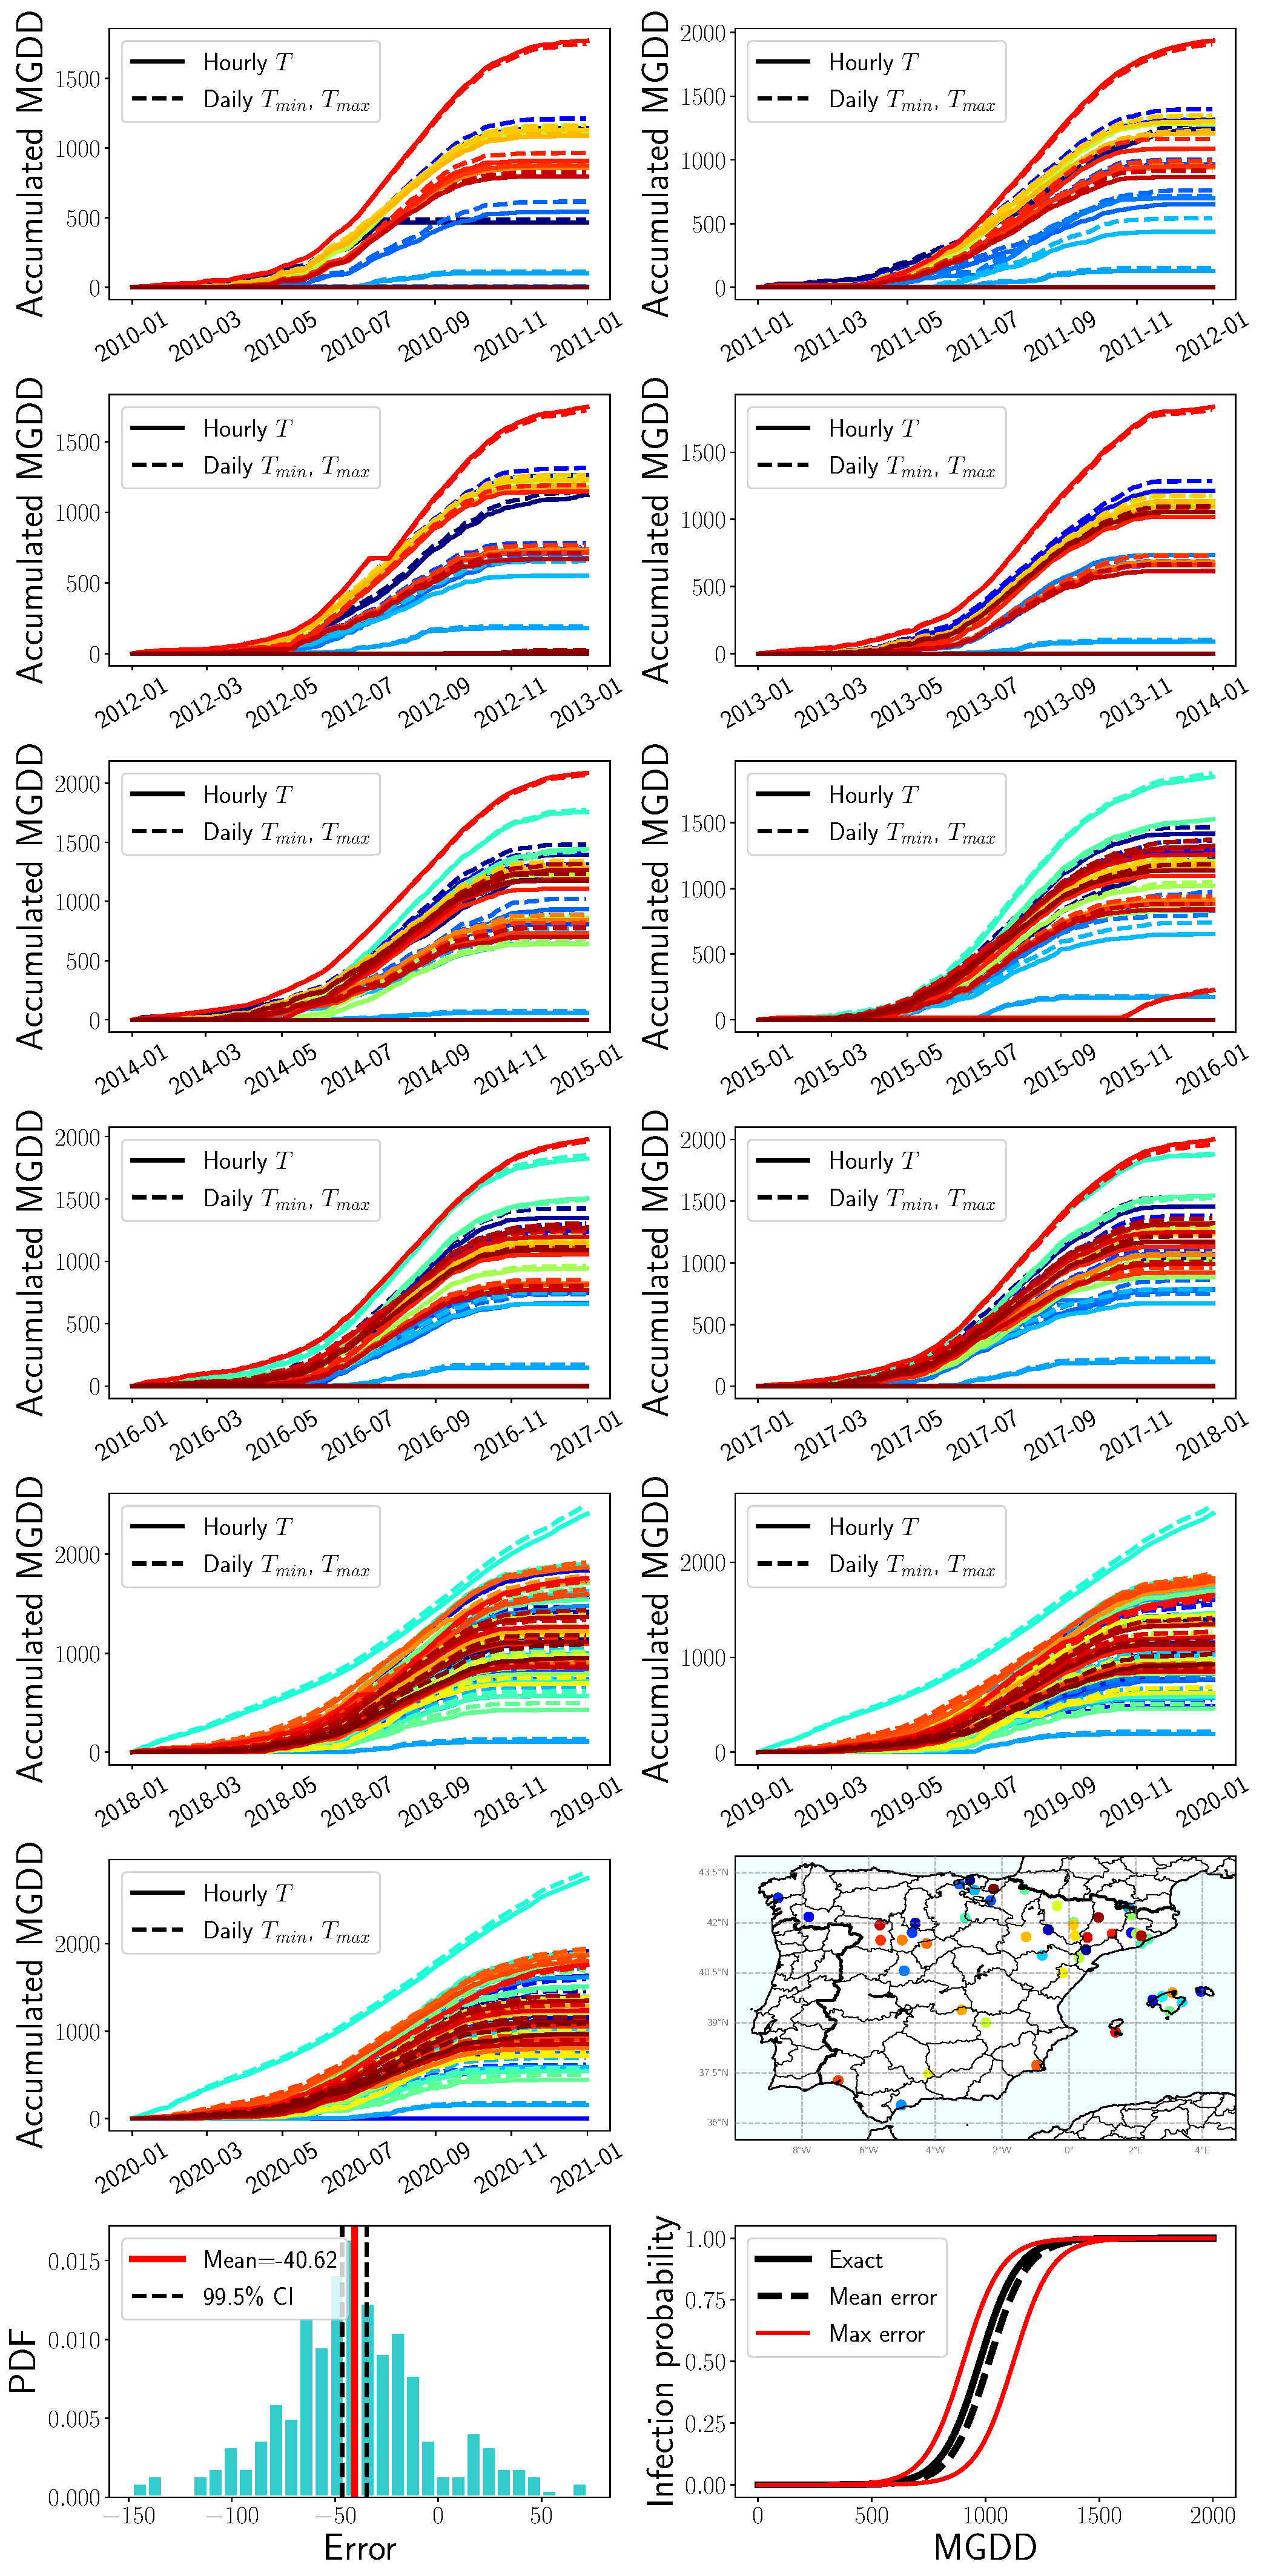
\includegraphics[width=0.64\textwidth]{Figures/MGDD_approx_comparison.pdf}
    \caption{Comparison of MGDD accumulation computed with hourly mean
        temperature data (solid line) and daily maximum and minimum values
        (dashed
        line) using data from several meteorological stations in Spain and
        different
        years. The last row shows the distribution of errors and mean error in
        MGDD and
        the mean and maximum potential errors in infection probability.}
    \label{fig:MGDD_app}
\end{figure}

\begin{figure}[H]
    \centering
    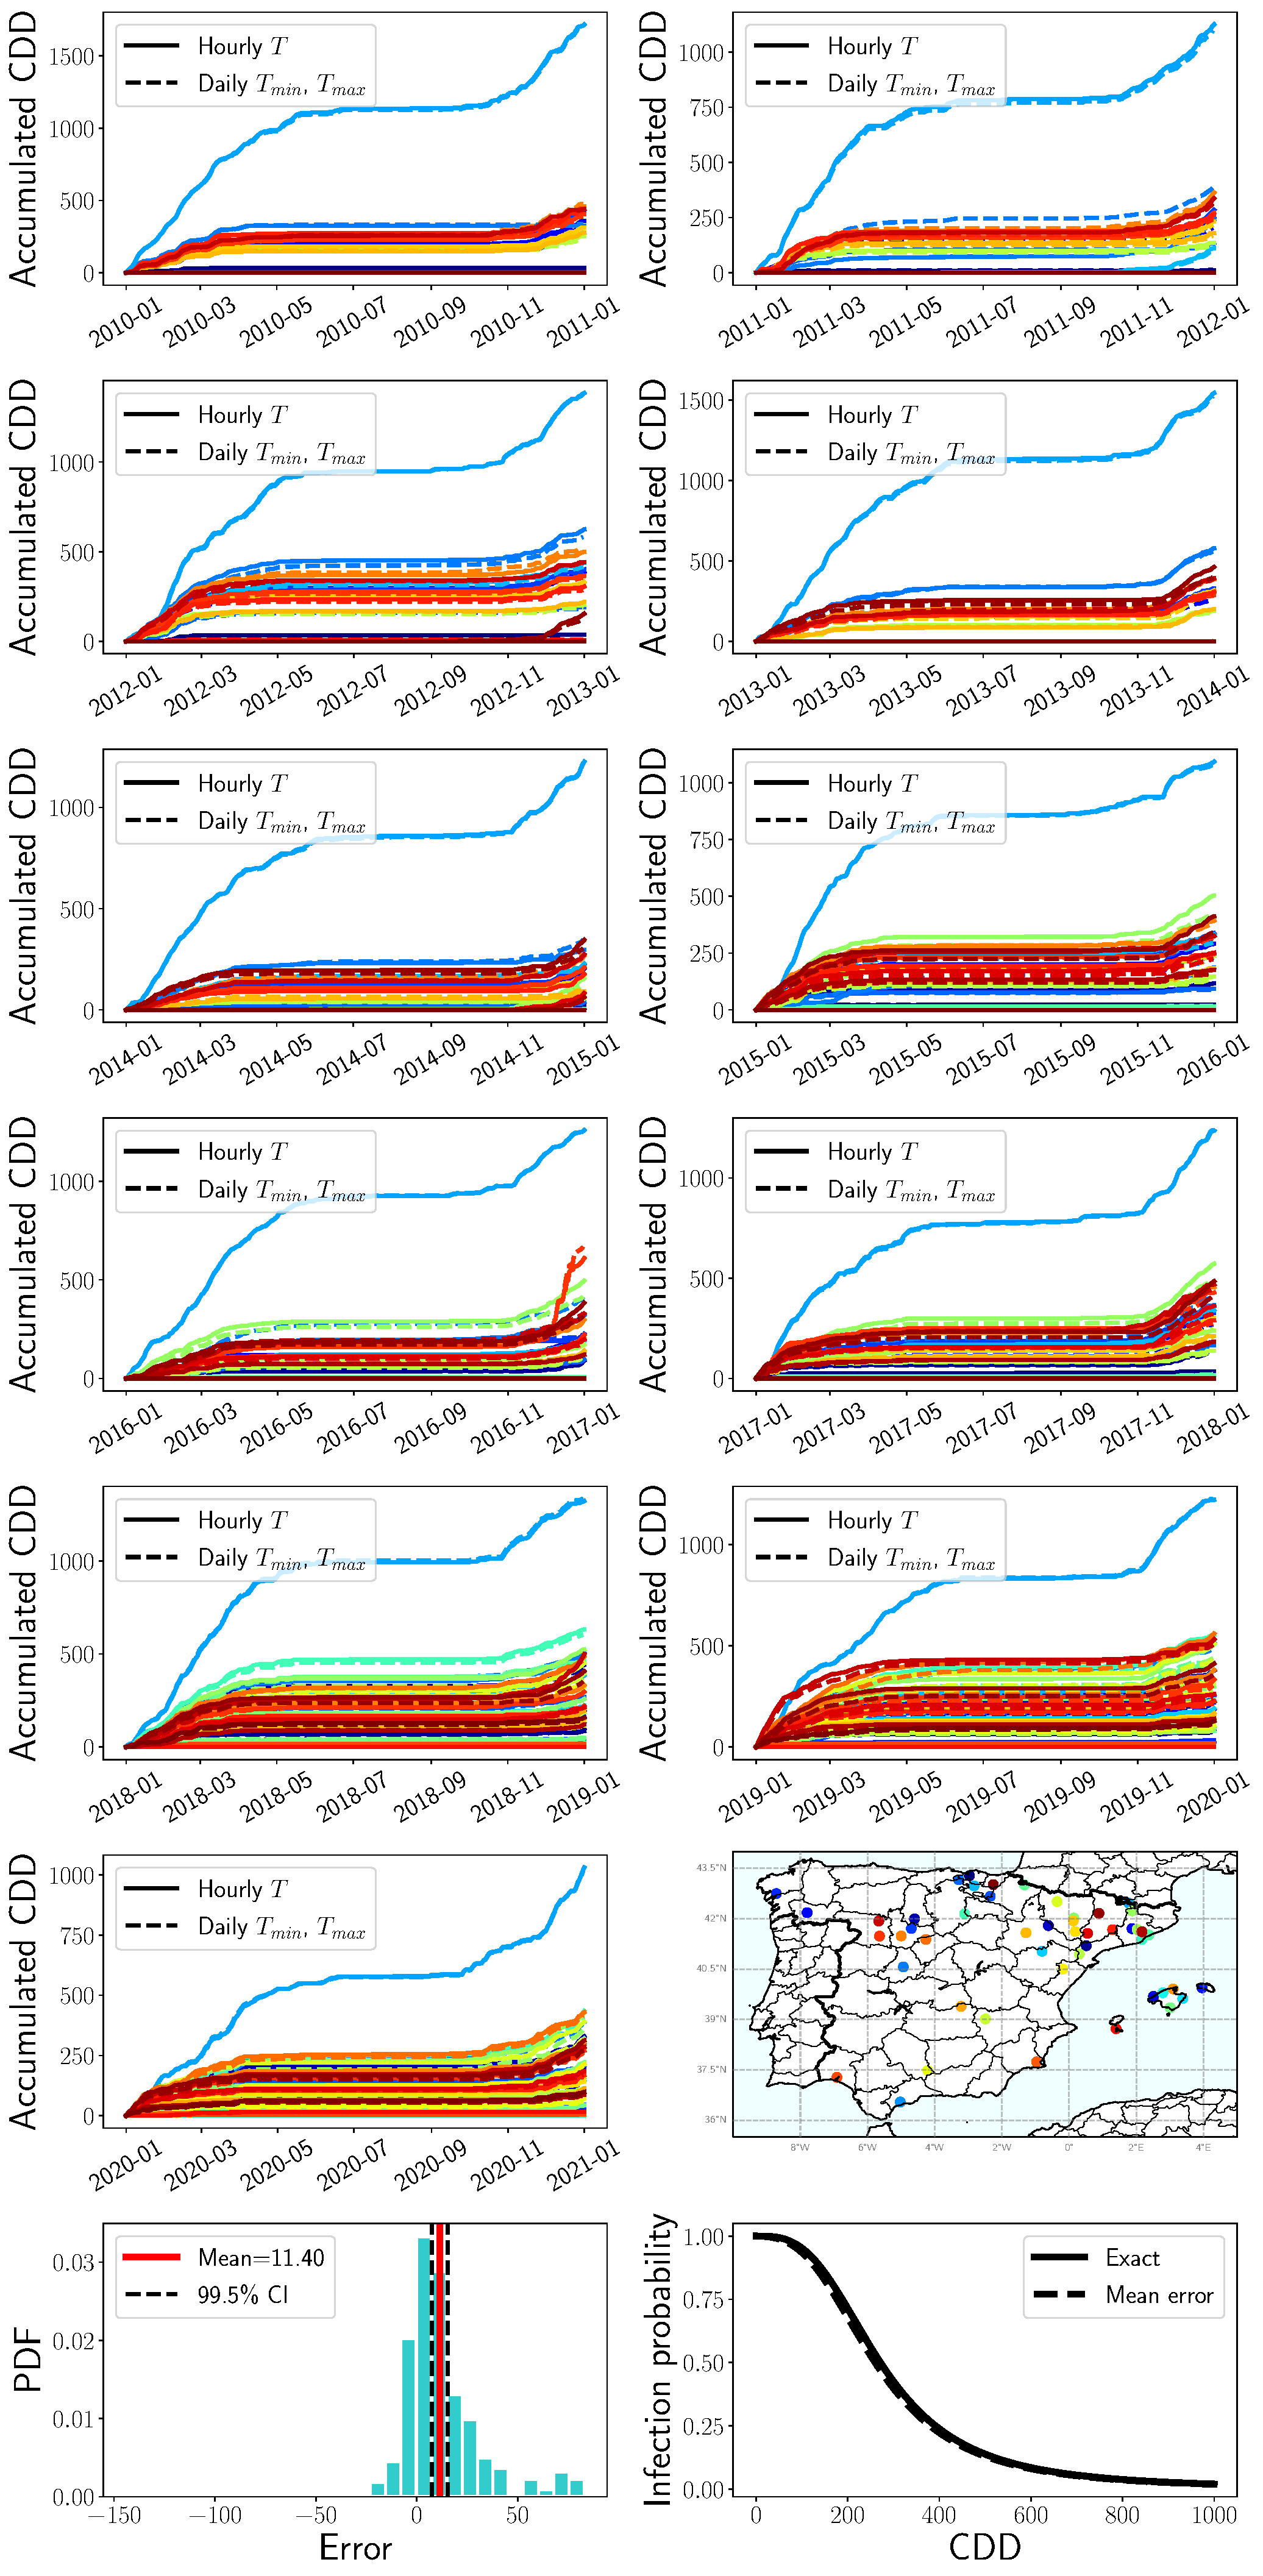
\includegraphics[width=0.64\textwidth]{Figures/CDD_approx_comparison.pdf}
    \caption{Comparison of CDD accumulation computed with hourly mean
        temperature data (solid line) and daily maximum and minimum values
        (dashed
        line) using data from several meteorological stations in Spain and
        different
        years. The last row shows the distribution of errors and mean error in
        CDD and
        the mean and maximum potential errors in infection probability.}
    \label{fig:CDD_app}
\end{figure}

\begin{figure}[H]
    \centering
    \includegraphics[width=\textwidth]{Figures/E-OBS_vs_ERA5.pdf}
    \caption{Differences in annual accumulated MGDD and CDD when using
        ERA5-Land dataset with hourly mean temperature and EOBS dataset with
        maximum
        and minimum daily temperatures.}
    \label{fig:EOBS_vs_ERA5}
\end{figure}

%%% High Resolution %%%
\section{The effect of spatial resolution on risk projections}

We compared the risk indices obtained with ERA5 (10 km resolution) and CHELSA
(1 km resolution) datasets in different viticulture areas. The results show
that the risk indices obtained with CHELSA are generally higher than those
obtained with ERA5, specially in river valleys and coastal areas, where the
temperature is more influenced by the local topography. This is particularly
evident in the Mediterranean basin or South Africa (\cref{fig:ERA5_vs_chelsa}).
We also compared the projected risk increase rate in different viticulture
areas, showing that the risk increase rate is generally higher in CHELSA than
in ERA5, with the exception of South America, where the risk increase rate is
similar in both datasets (\cref{fig:area_at_risk}).

\begin{figure}[H]
    \centering
    \includegraphics[width=1\textwidth]{Figures/area_risk.pdf}
    \caption{Difference in projected risk in increase rate based on CHELSA
        (high-resolution, 1 km) and ERA5 (mid-resolution, 10 km) datasets in
        global
        viticulture areas. (A) Europe (B) United States (C) South Africa (D)
        South
        America (E) Australia.}
    \label{fig:area_at_risk}
\end{figure}

\begin{figure}[H]
    \centering
    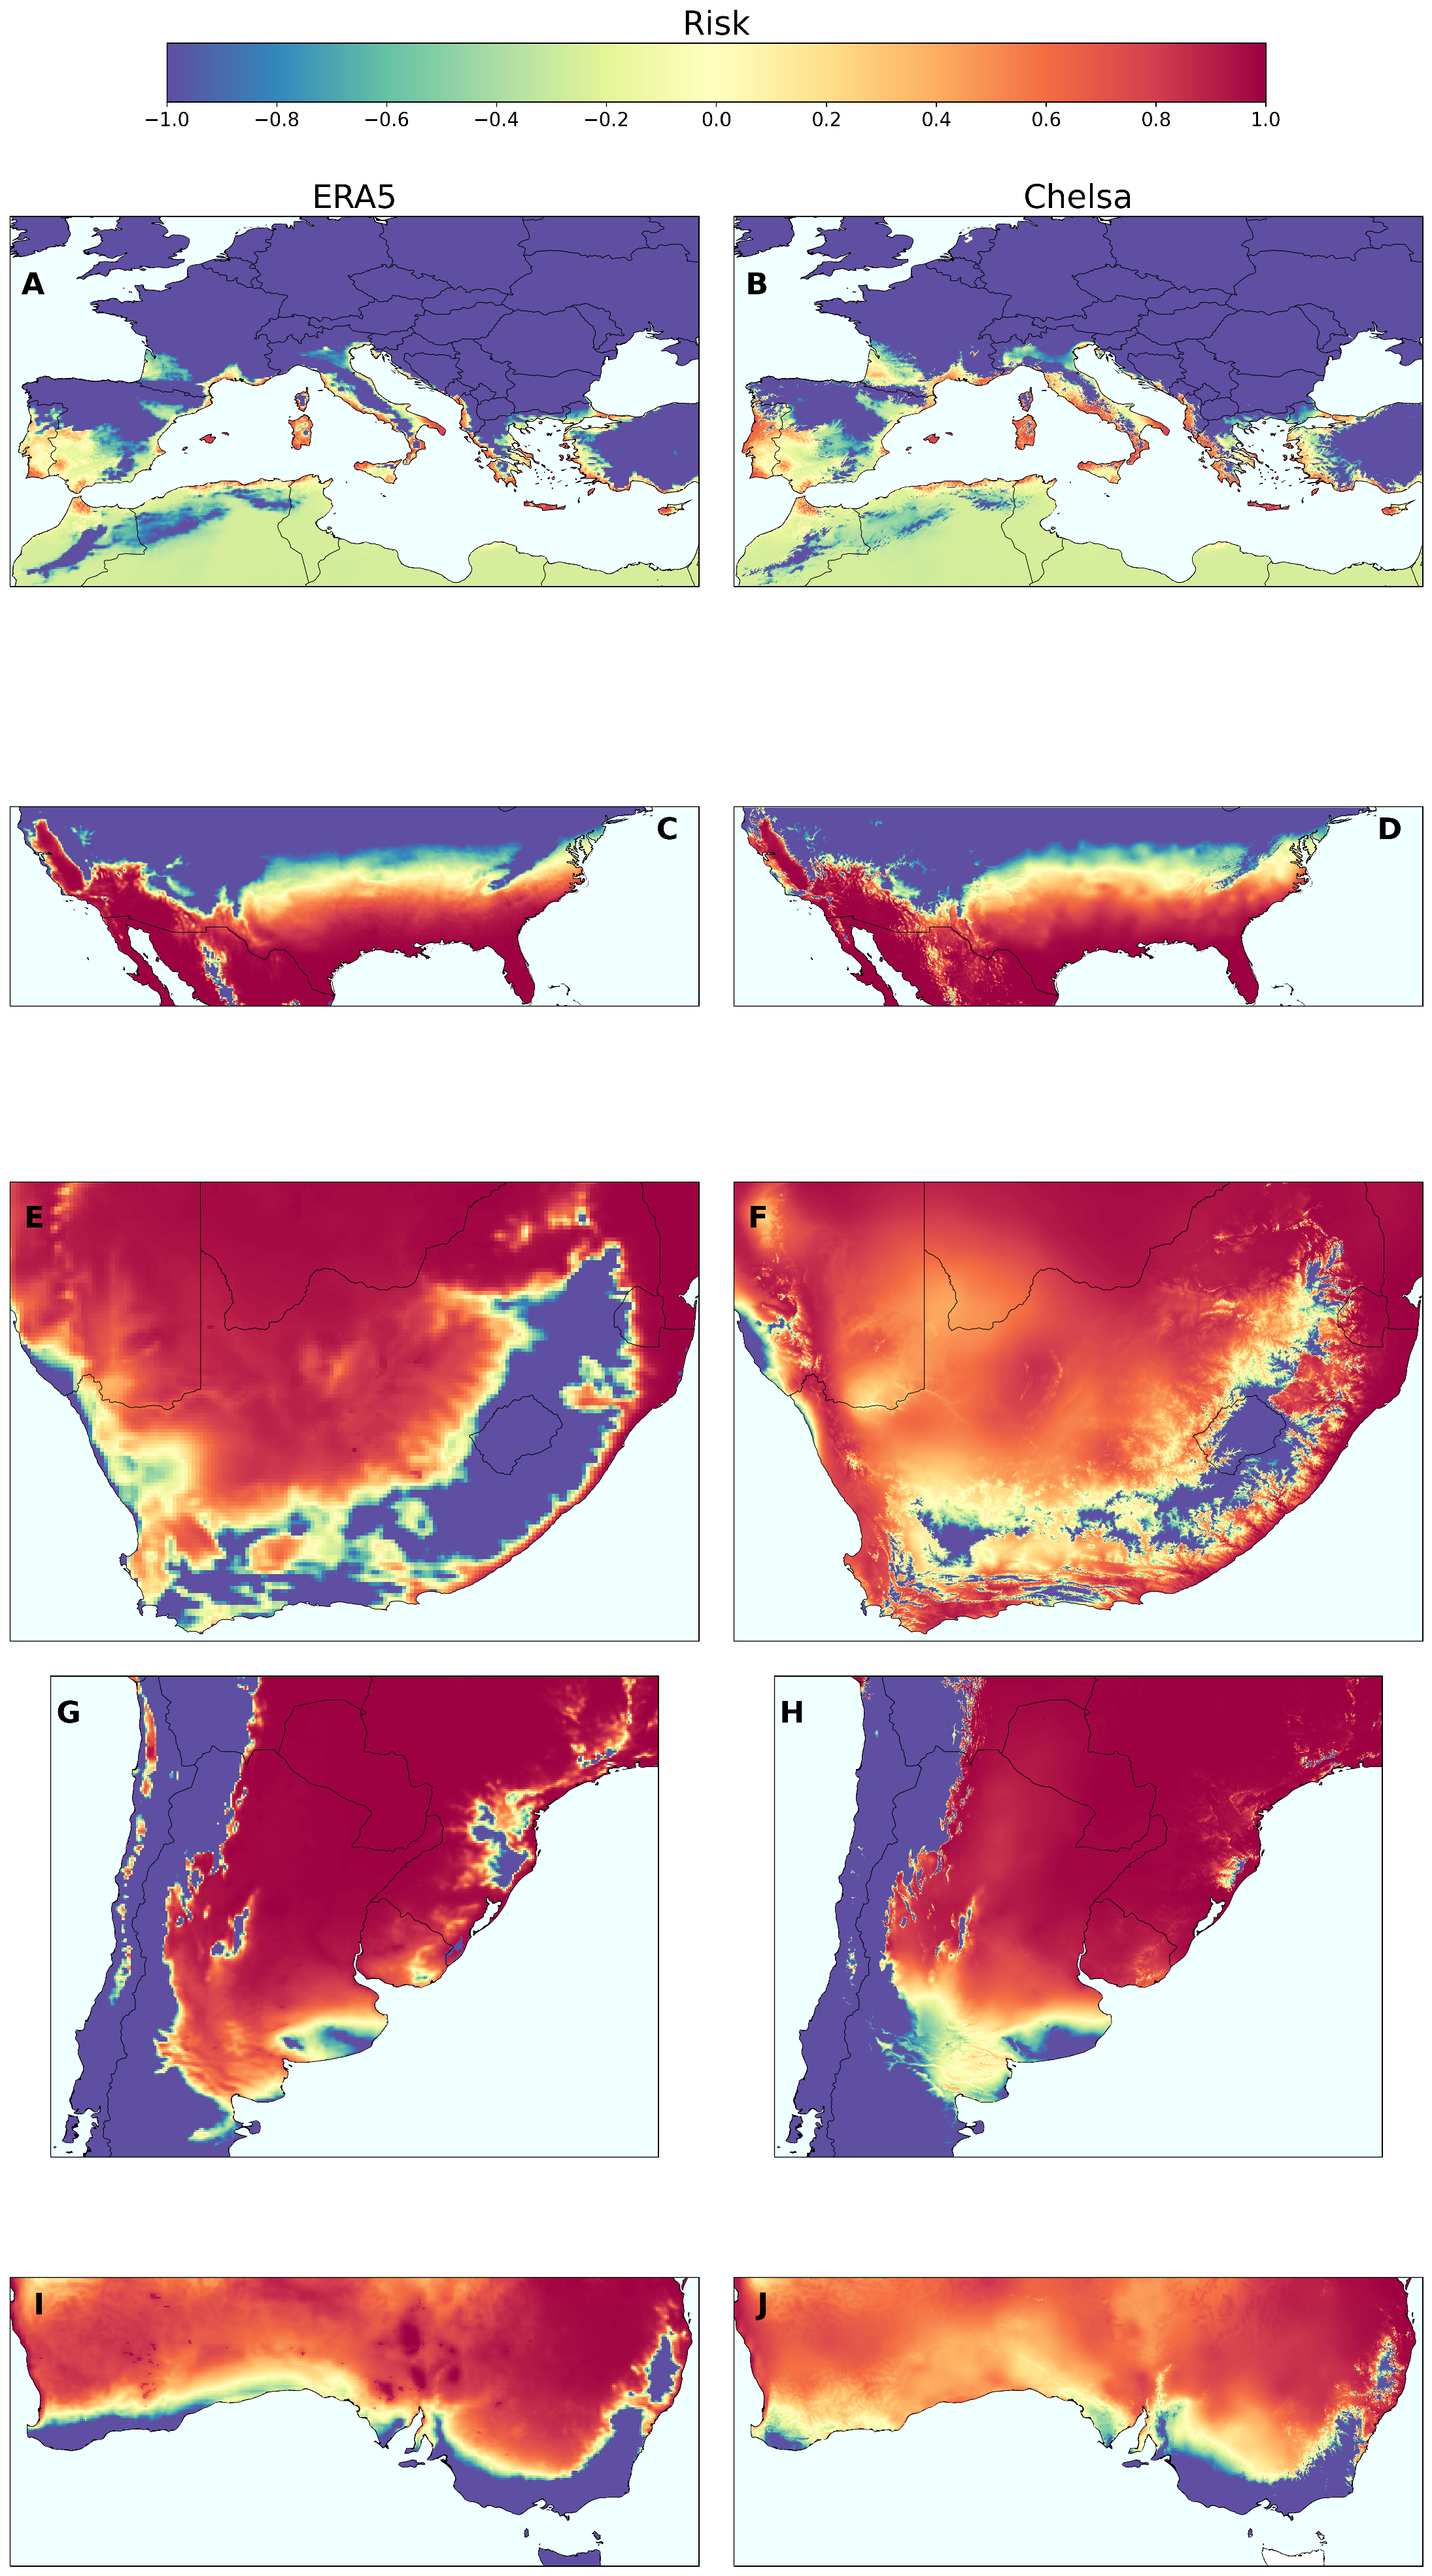
\includegraphics[width=0.75\textwidth]{Figures/ERA5_vs_Chelsa_SI.pdf}
    \caption{Comparison of risk indices obtained with ERA5 (mid-resolution
        -- 10 km, left column) and CHELSA (high-resolution -- 1 km, right
        column)
        datasets in Europe (A-B), United States (C-D), South Africa (E-F),
        South
        America (G-H) and Australia (I-J).}
    \label{fig:ERA5_vs_chelsa}
\end{figure}

\section{\textit{Vitis vinifera} global distribution}

\begin{figure}[H]
    \centering
    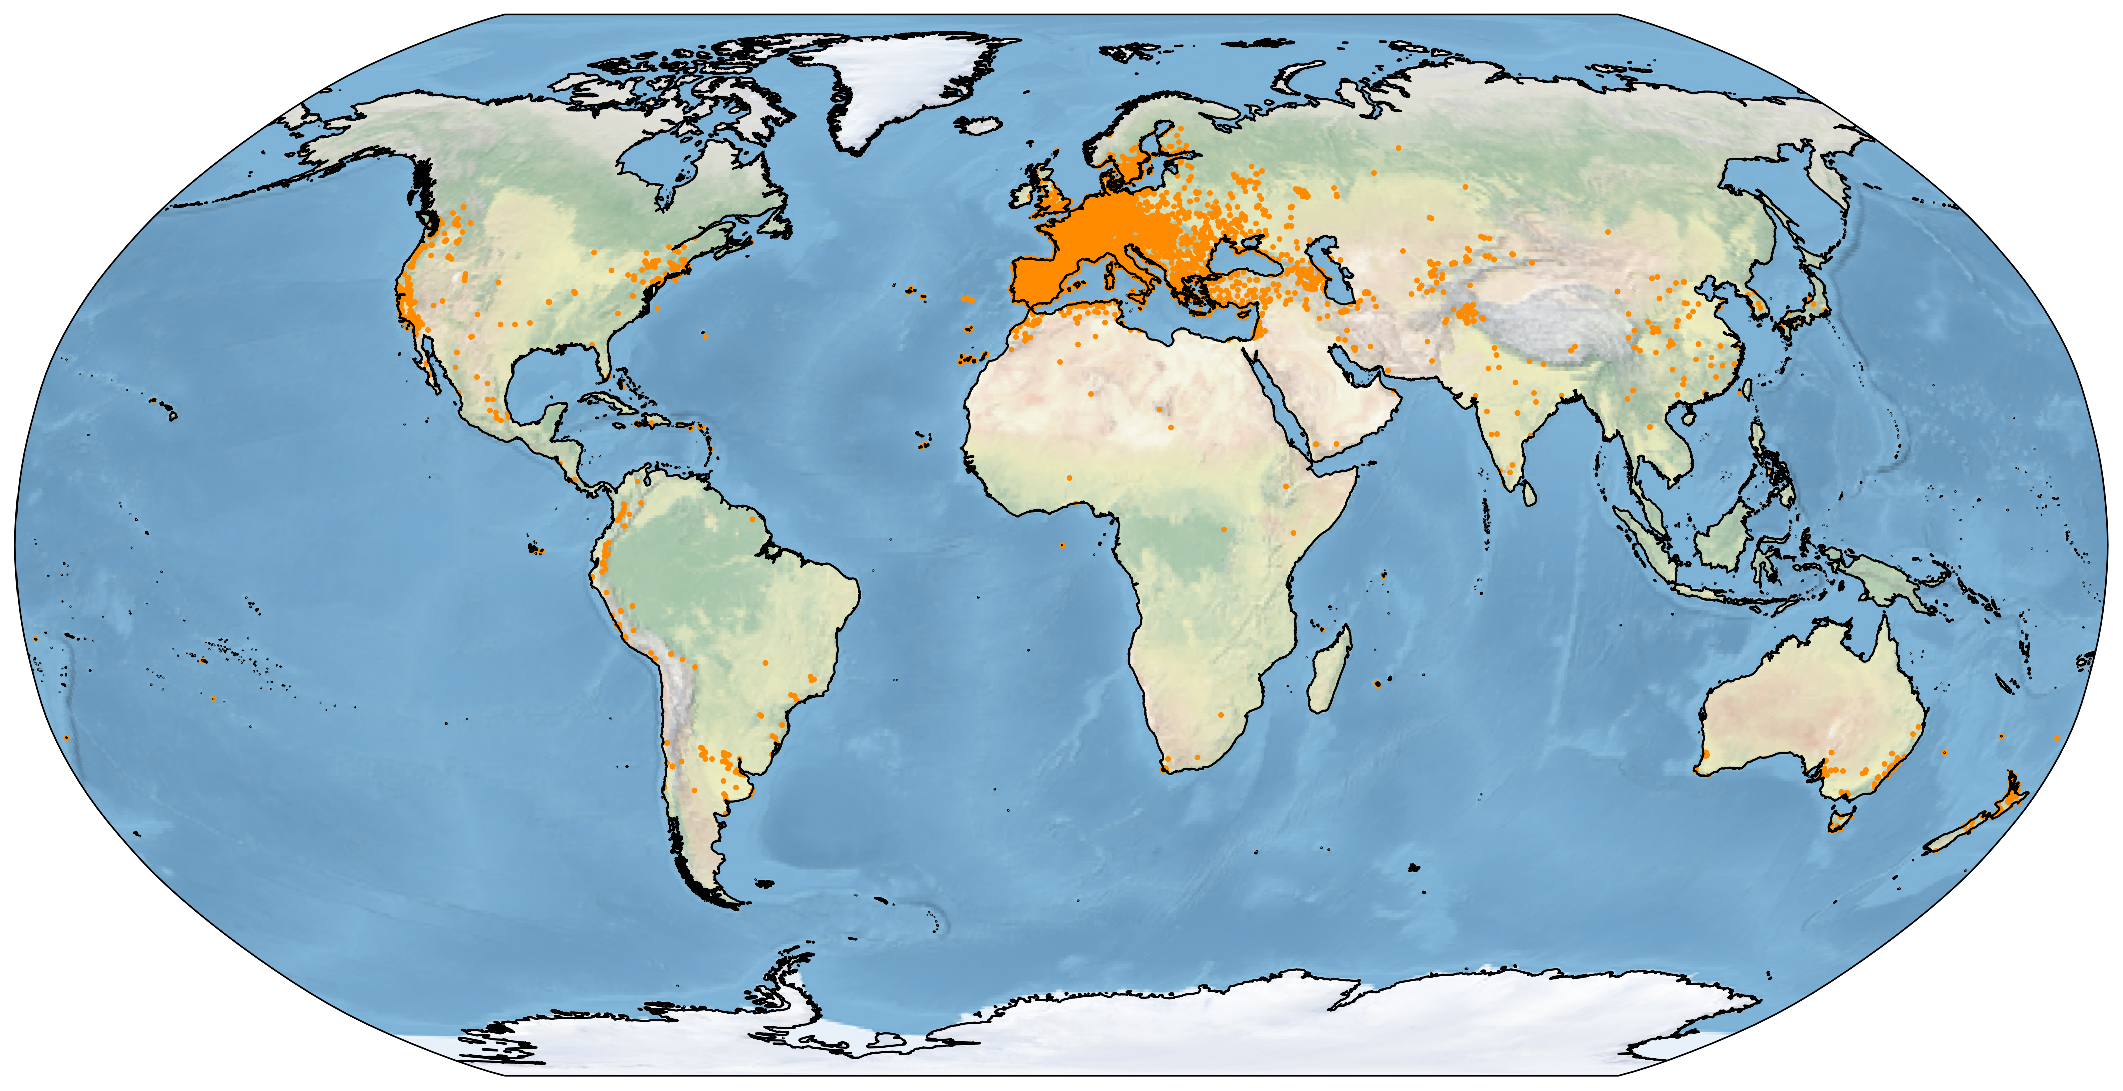
\includegraphics[width=\textwidth]{Figures/vid_locations.pdf}
    \caption{Presence locations of \textit{Vitis vinifera} obtained from
        GBIF.}
    \label{fig:vid_locations}
\end{figure}
